%%%%%%%%%%%%%%%%%%%%%%%%%%%%%%%%%%%%%%%%%%%%%%%%%%%%%%%%%%%%%%%%%%%%%%%%%
%
% File: operator_evolution.tex
%
% Author: A. J. Tropiano (tropiano.4@osu.edu)
% Date: August 23, 2019
%
% Draft of paper on SRG operator evolution and the Magnus expansion.
%
% Revision history:
%	08/28/19 --- Started outlining and added pieces from old notes.
%	09/09/19 --- Added more bullets to the introduction. Further organization.
%	09/19/19 --- Added more bullets to section 2.
%	09/27/19 --- Wrote the introduction and swapped the Magnus and operator sections.
%
%%%%%%%%%%%%%%%%%%%%%%%%%%%%%%%%%%%%%%%%%%%%%%%%%%%%%%%%%%%%%%%%%%%%%%%%%


\documentclass[preprintnumbers,floatfix,aps,prc,preprint,nofootinbib]{revtex4-1}

% Packages
\usepackage{amsmath}
\usepackage{amsfonts}
\usepackage{amssymb}
\usepackage{bm}
\usepackage[font=small,skip=0pt]{caption} % For captions on figures and tables
\usepackage{cellspace}
\usepackage{color}
\usepackage{enumerate}
\usepackage{epsfig}
\usepackage[figuresright]{rotating}
\usepackage{float}
\usepackage{hyperref} % For clickable links to sections within table of contents
\usepackage{graphicx}
\graphicspath{{../../Figures/}} % Setting the graphics path
\usepackage{physics} % For bra-ket notation
\usepackage{siunitx}
\usepackage[caption=false]{subfig} % For sub-figures

\newcommand{\eps}{\varepsilon}


\begin{document}


%%%%%%%%%%%%%%%%%%%%%%%%%%%%%%%%%%%%%%%%%%%%%%%%%%%%%%%%%%%%%%%%%%%%%%%%%
\title{Operator evolution from the similarity renormalization group and the Magnus expansion}


\author{A.~J.~Tropiano$^{1}$, S.~K.~Bogner$^{2}$, R.~J.~Furnstahl$^{1}$}

\affiliation{%
$^1$\mbox{Department of Physics, The Ohio State University, Columbus, OH 43210, USA}  \\
$^2$\mbox{National Superconducting Cyclotron Laboratory and Department of Physics and Astronomy,}  \\
\mbox{Michigan State University, East Lansing, MI 48824, USA}
}

\date{\today}

\begin{abstract}

\noindent{Ideas for Magnus / SRG operator evolution paper}
\\
-- SRG/Magnus evolution in different potentials (non-local, local, semi-local). Universality. High cutoffs.
\\
-- Block-diagonal generator for high cutoff potentials and operator evolution. How the block-diagonal generator handles spurious bound states.
\\
-- Testing the Magnus expansion for high cutoff potentials using the potentials from Wendt 2011 for comparison. Spurious bound states and connection to intruder states in IMSRG calculations.
\\
-- Operator evolution for different potentials and generators.

\end{abstract}

\maketitle

\newpage


%%%%%%%%%%%%%%%%%%%%%%%%%%%%%%%%%%%%%%%%%%%%%%%%%%%%%%%%%%%%%%%%%%%%%%%%%
\section{Introduction}
\label{sec:intro}

% Be more up front with motivation/purpose of the paper.
\noindent{%
\textbf{NN interaction and SRG decoupling.}
}
\\
The nuclear many-body problem has long been hindered by the short-range repulsive core and strong tensor force in nucleon-nucleon (NN) interactions leading to non-perturbative few- and many-body systems and strongly correlated wave functions. The Fourier transform of NN interactions gives rise to the coupling of low- and high-momentum modes, which is manifested as non-zero off-diagonal potential matrix elements. It is very difficult to implement these interactions in many-body methods using basis expansions, because the matrix dimension becomes too large for accurate calculations. Renormalization group (RG) methods can be used to soften the interaction to make many-body methods feasible. One such method, the similarity renormalization group (SRG), allows for a continuous change in resolution of the potential without changing the observables. More generally, the SRG can evolve any operator and wave function for consistent calculation of observables.
\\

\noindent{%
\textbf{SRG formalism}
}
\\
The SRG decouples low- and high-momentum scales by applying a continuous unitary transformation $U(s)$ where $s=0 \rightarrow \infty$ is the flow parameter. The evolved operator is given by
%
\begin{eqnarray}
	\label{eq:srg_operator}
	O(s) = U(s) O(0) U^{\dagger}(s),
\end{eqnarray}
%
where $O(0)$ corresponds to the initial operator. Because $U(s)$ is unitary, the observables of the operator are preserved. In practice, the unitary transformation U(s) is not explicitly solved for; the evolved operator is given by solving a differential flow equation which is obtained by taking the derivative of Eqn. (\ref{eq:srg_operator}),
%
\begin{eqnarray}
	\label{eq:srg_flow}
	\frac{dO(s)}{ds} = [\eta(s), O(s)],
\end{eqnarray}
%
where $\eta(s)=\frac{dU(s)}{ds} U^{\dagger}(s) = -\eta^{\dagger}(s)$ is the anti-hermitian SRG generator. The generator is defined as a commutator, $\eta(s) = [G, H(s)]$, where $G$ specifies the type of flow. The choice in $G$ determines the pattern of decoupling in the operator. By setting $G=H_D(s)$, the diagonal of the Hamiltonian, the operator is driven to band-diagonal form. This choice was implemented by Wegner in condensed matter physics \cite{Wegner:1994ab}. In a similar option used in nuclear physics, $G$ is set to the relative kinetic energy, $T_{rel}$, which also drives to band-diagonal form. In most cases, these two choices give the same evolved operators. In exceptional cases, which will be discussed later in the paper, the two band-diagonal choices can have drastically different behavior. For band-diagonal decoupling, it is convenient to define $\lambda \equiv s^{-1/4}$ which roughly measures the width of the band-diagonal in the decoupled operator. For block-diagonal decoupling, $G=P H(s) P + Q H(s) Q \equiv H_{BD}(s)$, where $P$ and $Q$ are low- and high-momentum projection operators, the operator is split into low- and high-momentum sub-blocks by specifying a separation in momentum $\Lambda$. These transformations are similar to V\textsubscript{low k} transformations \textcolor{red}{(references?)} but keep the high-momentum matrix elements non-zero, although entirely decoupled from the low-momentum sub-block. Generally the flow equation (\ref{eq:srg_flow}) is solved up to some finite value of $s$ with a high-order ODE solver. For notational convenience, we write the generators without the $s$ dependence in the rest of the paper.
\\

\noindent{%
\textbf{Background on modern nuclear potentials and universality.}
}
\\
There has been tremendous progress in development of NN interactions from chiral effective field theory ($\chi^{EFT}$) in the last decade. Previous SRG studies were limited to phenomenological interactions or some of the first non-local chiral interactions \cite{Entem:2003ft}, but with much more variance in modern chiral interactions, we would like to revisit the question of how different potentials and other operators change under SRG transformations. Since $\chi^{EFT}$ is an effective field theory, different potentials will still give the same $S$-matrix, that is, the potentials are phase equivalent up to some higher energy. However, the potentials themselves can differ in many ways such as the regulator functions, cutoff, order, and so forth, and thus, the potential matrix elements are not the same. Dainton \textit{et al.} \cite{Dainton:2013axa} demonstrated SRG transformations drive different NN potentials to the same low-momentum matrix elements, that is, a flow to universality up to the momentum value of phase inequivalence. We address the question of universality for modern chiral potentials as well as how other operators change with respect to the corresponding SRG transformations.
\\

\noindent{%
\textbf{High cutoffs}
}
\\
There has also been renewed interest in studying chiral interactions at high cutoffs \cite{Tews:2018sbi}. In spin-triplet channels and at leading-order (LO), taking the cutoff to high values can result in spurious, deeply bound states from a highly singular short-ranged tensor force. In principle, these deep bound states are outside the range of the EFT and are absorbed by counterterms at higher order. In \cite{Wendt:2011qj}, it was shown that band-diagonal SRG decoupling of NN potentials in partial waves with spurious bound states changes significantly depending on the choice of SRG generator. These high cutoff potentials provide a unique opportunity to understand some of the previous points about universality, the choice of SRG generator and decoupling, as well as a good test problem for a variant of the SRG, which utilizes the Magnus expansion \cite{Morris:2015yna}.
\\

\noindent{%
\textbf{The Magnus expansion}
}
\\
The Magnus expansion gives the SRG the capability to solve for the unitary transformation explicitly which can then be applied to any other operator of interest. This offers a huge numerical simplification in Fock-space where the matrix size of operators can become very large. The Magnus expansion is often used in in-medium SRG (IMSRG) calculations to solve the nuclear many-body problem directly. In some IMSRG calculations, intruder states can shift to the energy scale of the reference state in valence-space and severely distort low-energy properties. It is not understood how the IMSRG procedure evolves intruder state systems. Due to the prominence of the Magnus expansion in IMSRG, one must first understand if the Magnus approach matches the typical approach for difficult systems before investigating the intruder state problem. For this reason, NN potentials with spurious bound states offer a good test laboratory for the Magnus implementation to better understand if the Magnus is equivalent to the SRG approach.
\\

\noindent{%
\textbf{Overview of sections.}
}


%%%%%%%%%%%%%%%%%%%%%%%%%%%%%%%%%%%%%%%%%%%%%%%%%%%%%%%%%%%%%%%%%%%%%%%%%
\section{SRG evolution of NN potentials}
\label{sec:srg_evolution_nn_potentials}


% Summarize what we're looking at in this section and general conclusions. What did I not cover in the introduction?
%
\noindent{%
\textbf{General outline of the section}
}
\\
-- Comparison of potential evolution with different potentials and SRG generators.
\\
-- Universality.
\\
\textbf{Analysis of figures}
\\
-- Fig.~\ref{fig:potential_contours_RKE_Wegner} illustrates the SRG in a nutshell. Here, we evolve three partial wave channels of RKE N$^3$LO \cite{Reinert:2017usi} where the cutoff $\Lambda=450$ MeV to $\lambda=1.5$ fm$^{-1}$. We see that the off-diagonal elements of the potential approach zero and the potential is driven to band-diagonal form.
%
\begin{figure}[H]
	\centering
	\subfloat[]{%
	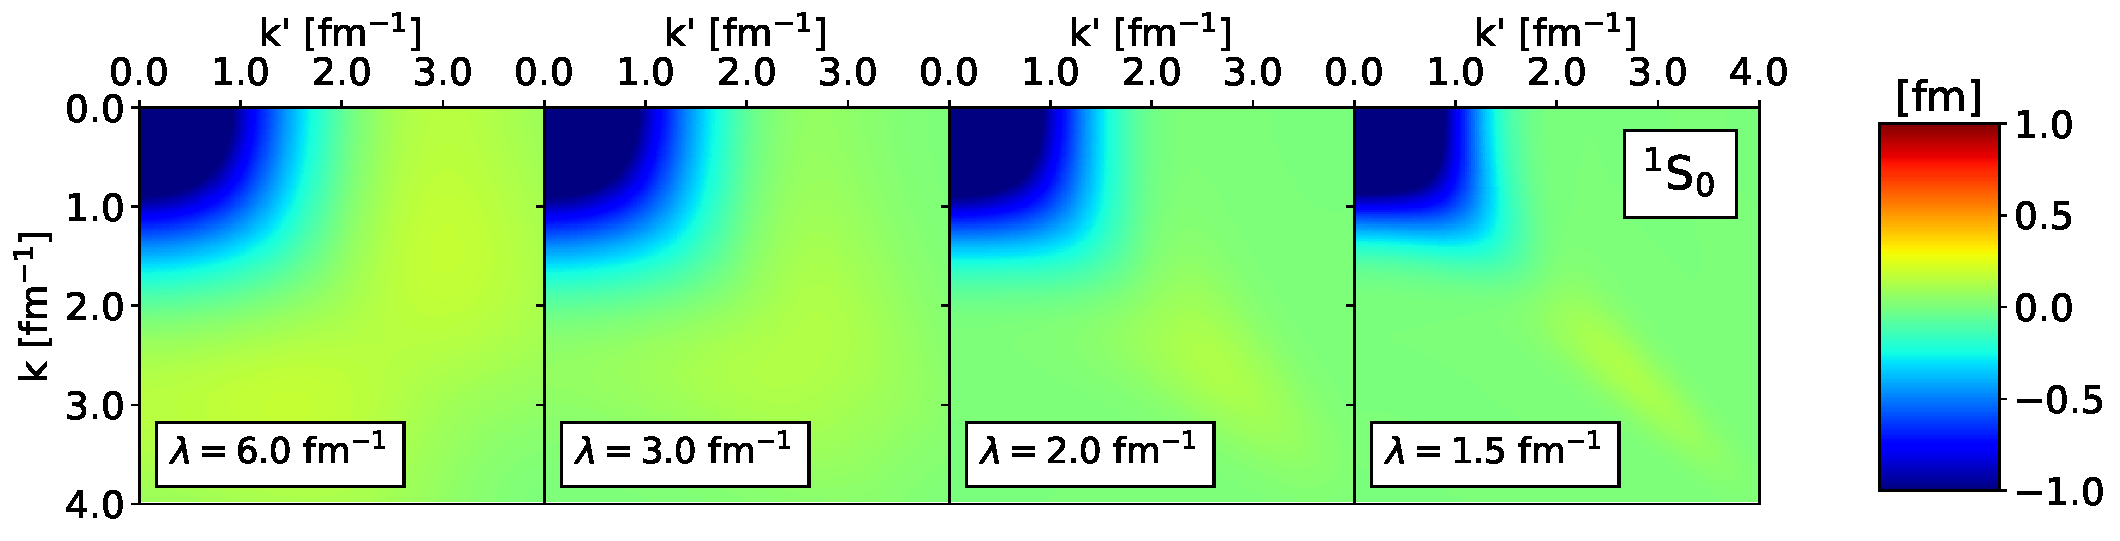
\includegraphics[clip,width=0.9\columnwidth]{SRG_potentials/potential_contours_kvnn106_1S0_Wegner_channel_label}%
	}
	
	\subfloat[]{%
	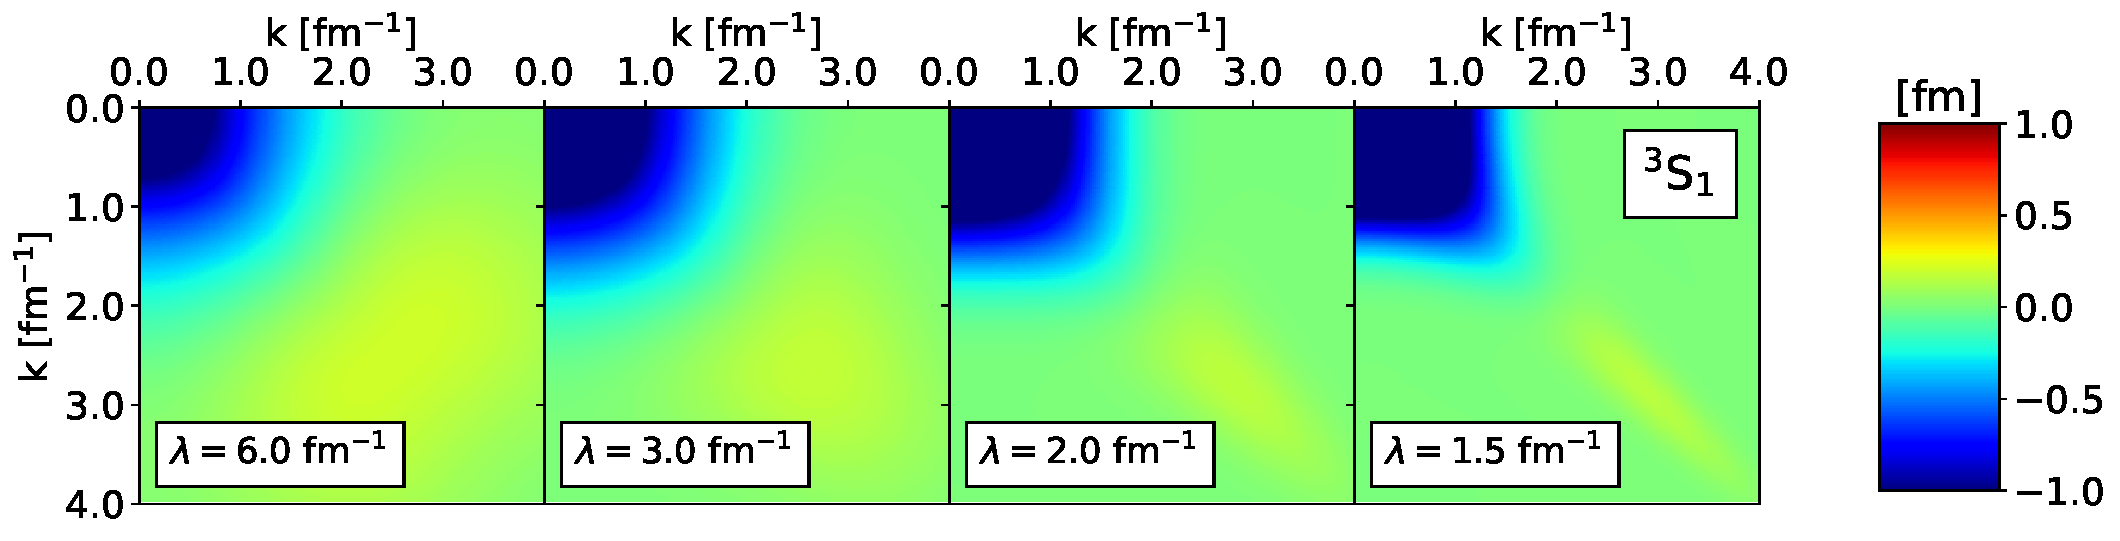
\includegraphics[clip,width=0.9\columnwidth]{SRG_potentials/potential_contours_kvnn106_3S1_Wegner_channel_label}%
	}

	\subfloat[]{%
	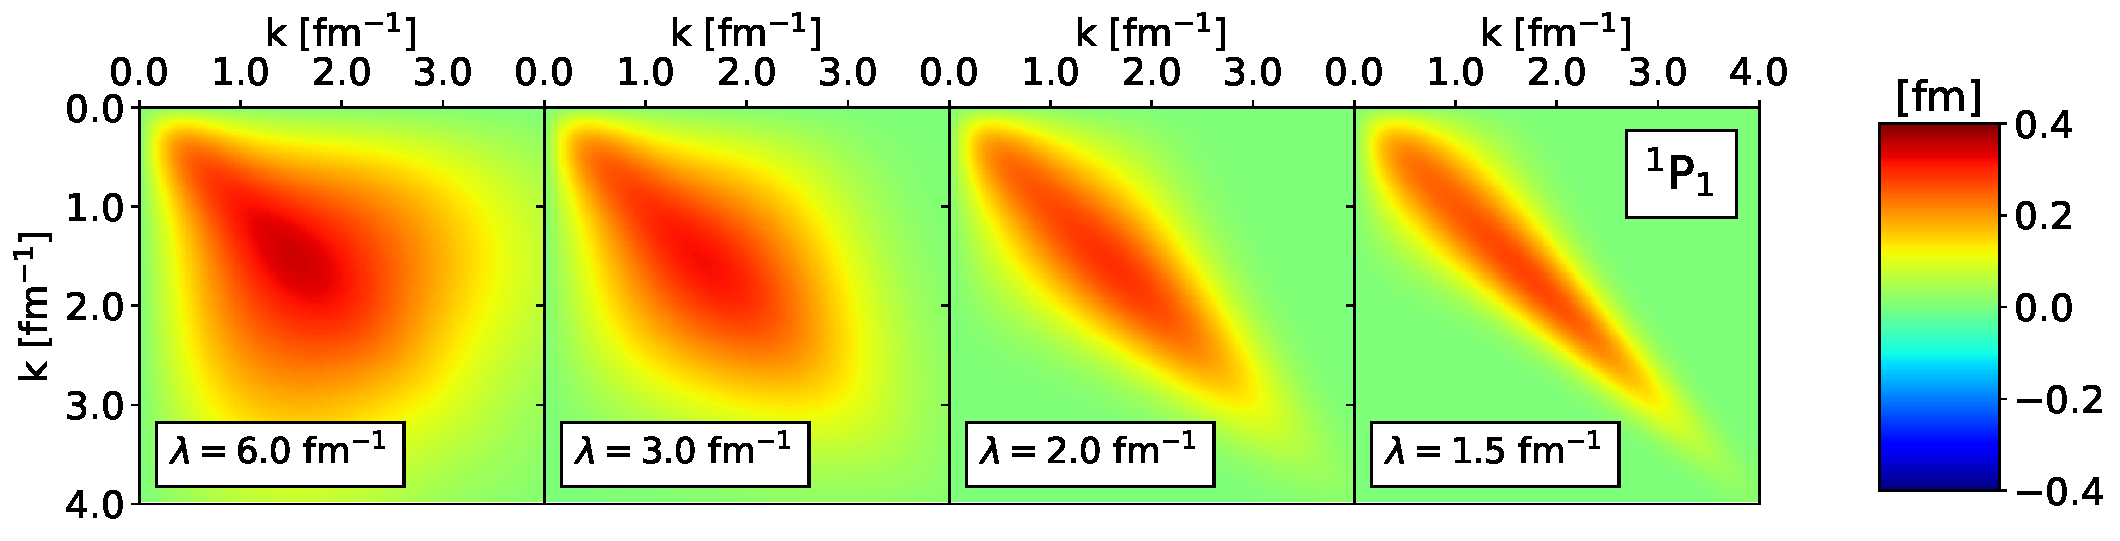
\includegraphics[clip,width=0.9\columnwidth]{SRG_potentials/potential_contours_kvnn106_1P1_Wegner_channel_label}%
	}
	\caption{Matrix elements of the RKE N$^3$LO potential SRG-evolving in $\lambda$ right to left under transformations with the Wegner generator in the $^1$S$_0$ (a), $^3$S$_1$ (b), and $^1$P$_1$ (c) channels.}
	\label{fig:potential_contours_RKE_Wegner}
\end{figure}
%
\noindent{%
-- In Fig.~\ref{fig:potential_contours_3S1_Wegner} we consider three different SRG-evolved potentials in the $^3$S$_1$ channel: EM N$^3$LO (500 MeV cutoff) \cite{Entem:2003ft}, RKE N$^3$LO (450 MeV cutoff) \cite{Reinert:2017usi}, and Gezerlis et al. N$^2$LO (1 fm cutoff) \cite{Gezerlis:2014zia}. The major difference in these three potentials are the regulator functions in the contact and pion-exchange terms. The EM N$^3$LO interaction is a non-local potential where both contact and pion-exchange interactions feature a non-local regulator function of the form exp$[-(p/\Lambda)^{2n}-(p'/\Lambda)^{2n}]$, where $\Lambda$ is the momentum-space cutoff and $n$ is an integer. However, a non-local regulator function for pion-exchange contributions can introduce regulator artifacts for cutoffs $\Lambda$ lower than the breakdown scale $\Lambda_b$. Several semi-local chiral potentials have been introduced to reduce regulator artifacts, such as the RKE N$^3$LO potential. Here, a local regulator function is applied for the long-range interactions in momentum-space, while a non-local regulator function is used for the short-range interactions. In some instances, non-local interactions are not suitable for $\textit{ab initio}$ approaches such as the quantum Monte Carlo (QMC) method motivating the need for fully local potentials. The Gezerlis et al. N$^2$LO potential is an example of a local interaction where the long-range terms have a local regulator function in coordinate-space and the short-range terms have a local regulator function in momentum-space.
}
\\
-- Takeaways from Fig.~\ref{fig:potential_contours_3S1_Wegner}: completely different at $\lambda=6$ fm$^{-1}$ but low-momentum matrix elements are similar at $\lambda=1$ fm$^{-1}$. Decoupled, low-momentum matrix elements are necessarily the same since the pion-exchange terms are calculated explicitly. (Cutoff dependence can play a role though for lower cutoffs.)
%
\begin{figure}[H]
	\centering
	\subfloat[]{%
	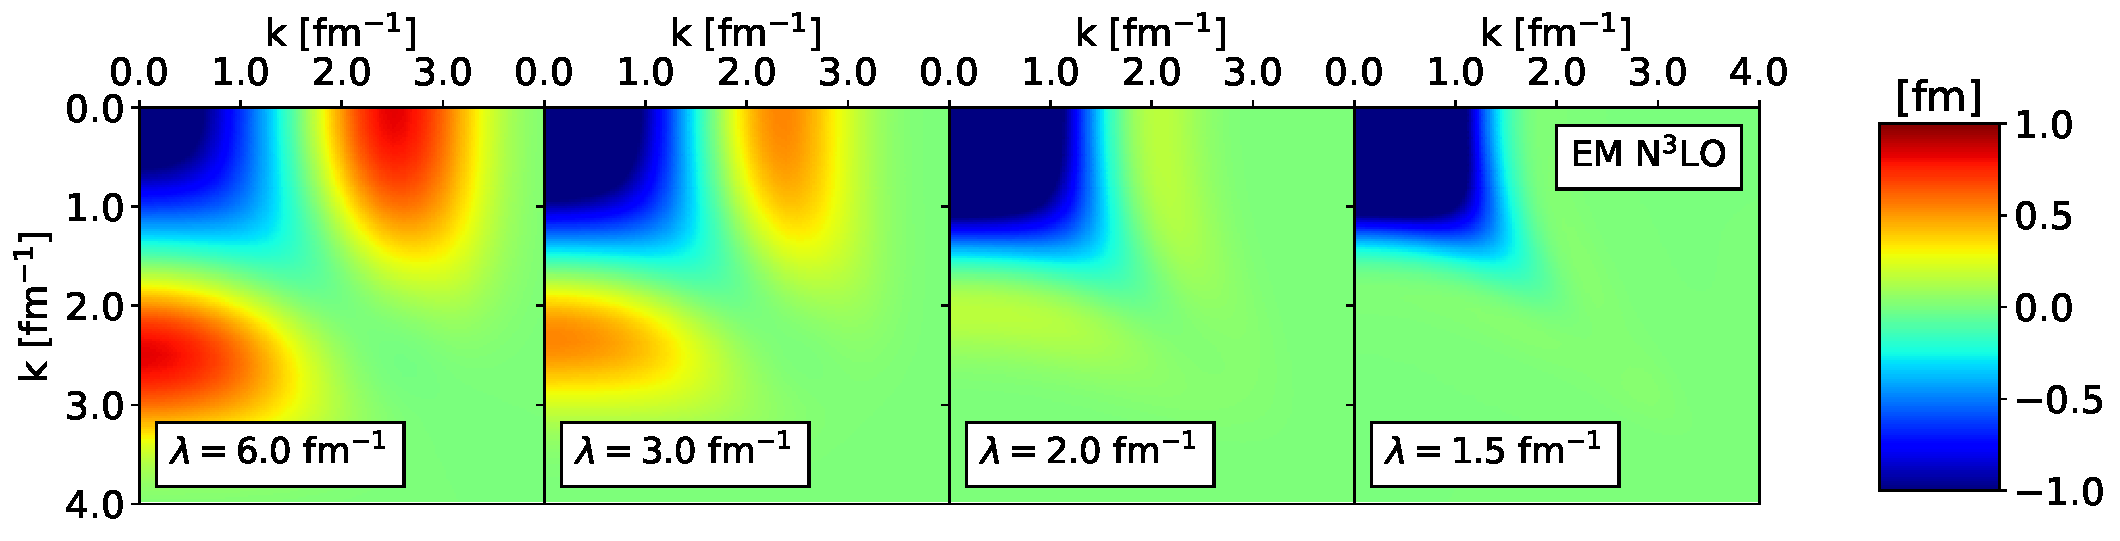
\includegraphics[clip,width=0.9\columnwidth]{SRG_potentials/potential_contours_kvnn10_3S1_Wegner_potential_label}%
	}
	
	\subfloat[]{%
	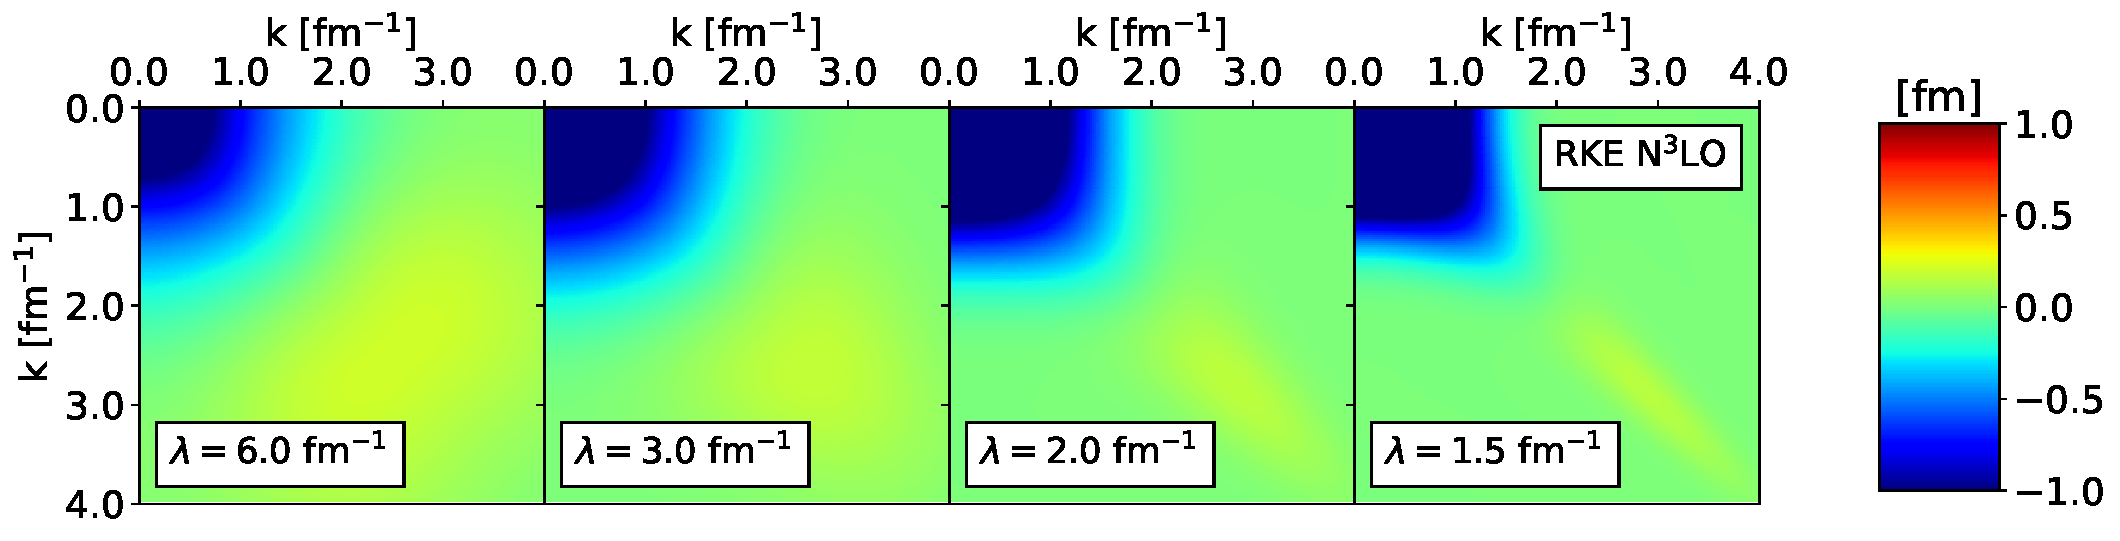
\includegraphics[clip,width=0.9\columnwidth]{SRG_potentials/potential_contours_kvnn106_3S1_Wegner_potential_label}%
	}

	\subfloat[]{%
	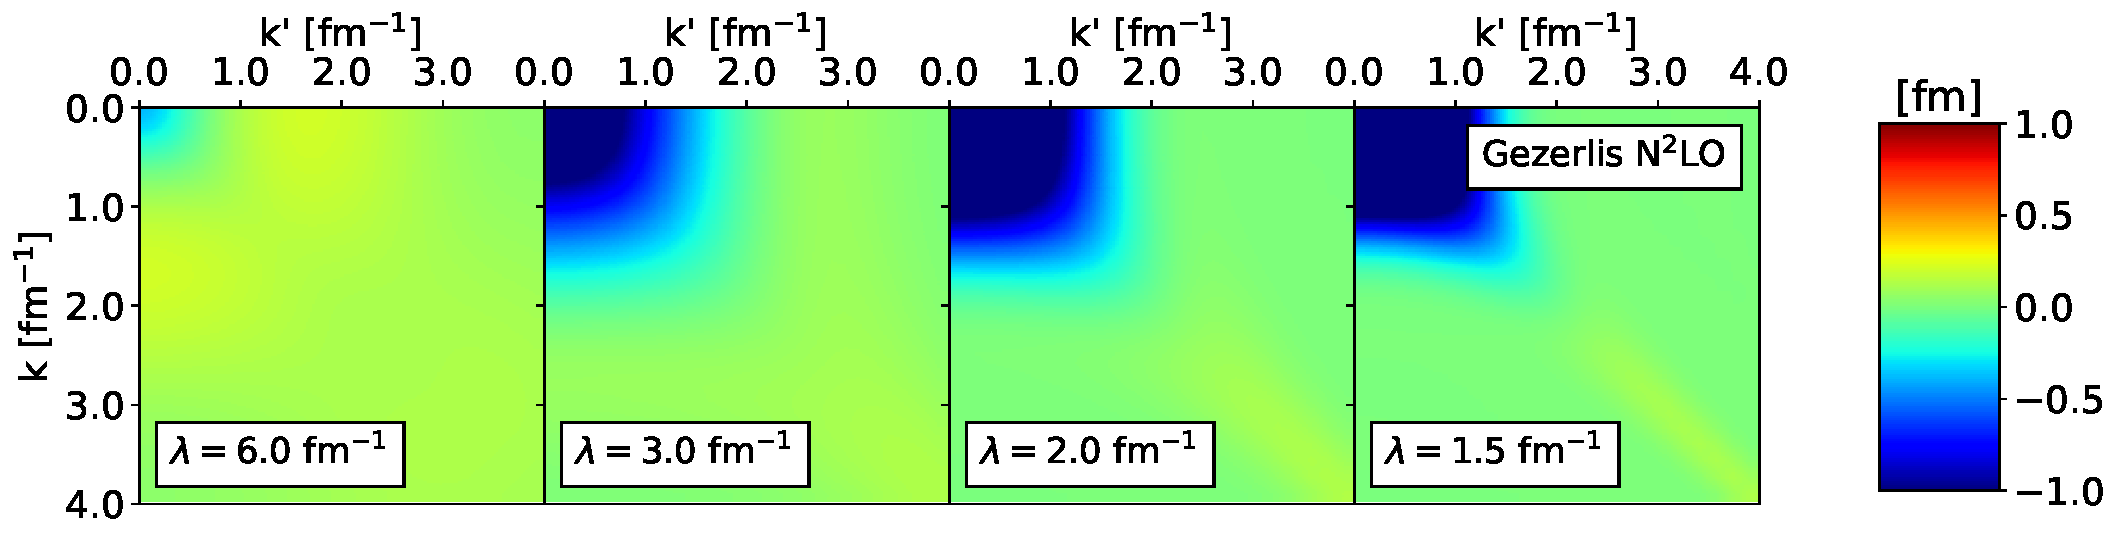
\includegraphics[clip,width=0.9\columnwidth]{SRG_potentials/potential_contours_kvnn222_3S1_Wegner_potential_label}%
	}
	\caption{Matrix elements of the EM N$^3$LO (a), RKE N$^3$LO (b), and Gezerlis et al. N$^2$LO (c) potentials SRG-evolving in $\lambda$ right to left under transformations with the Wegner generator in the $^3$S$_1$ channel.}
	\label{fig:potential_contours_3S1_Wegner}
\end{figure}
%
\noindent{%
-- Fig.~\ref{fig:potential_contours_3S1_RKE} shows the SRG-evolved RKE N$^3$LO (450 MeV cutoff) potential in the $^3$S$_1$ channel for two SRG generators: the Wegner and block-diagonal generators which drive the potential to band- and block-diagonal form, respectively. We continue to evolve to band-diagonal form with respect to the parameter $\lambda$, but for the block-diagonal generator, we label sub-plots with the parameter $\Lambda$ which characterizes the sharp cutoff in decoupling the low- and high-momentum matrix elements.
}
\\
-- Takeaways from Fig.~\ref{fig:potential_contours_3S1_RKE}: smooth decoupling for Wegner and sharp for block-diagonal, each unique generator should have its own type of universality. Check this more quantitatively by comparing matrix element ``slices''.
%
\begin{figure}[H]
	\centering
	\subfloat[]{%
	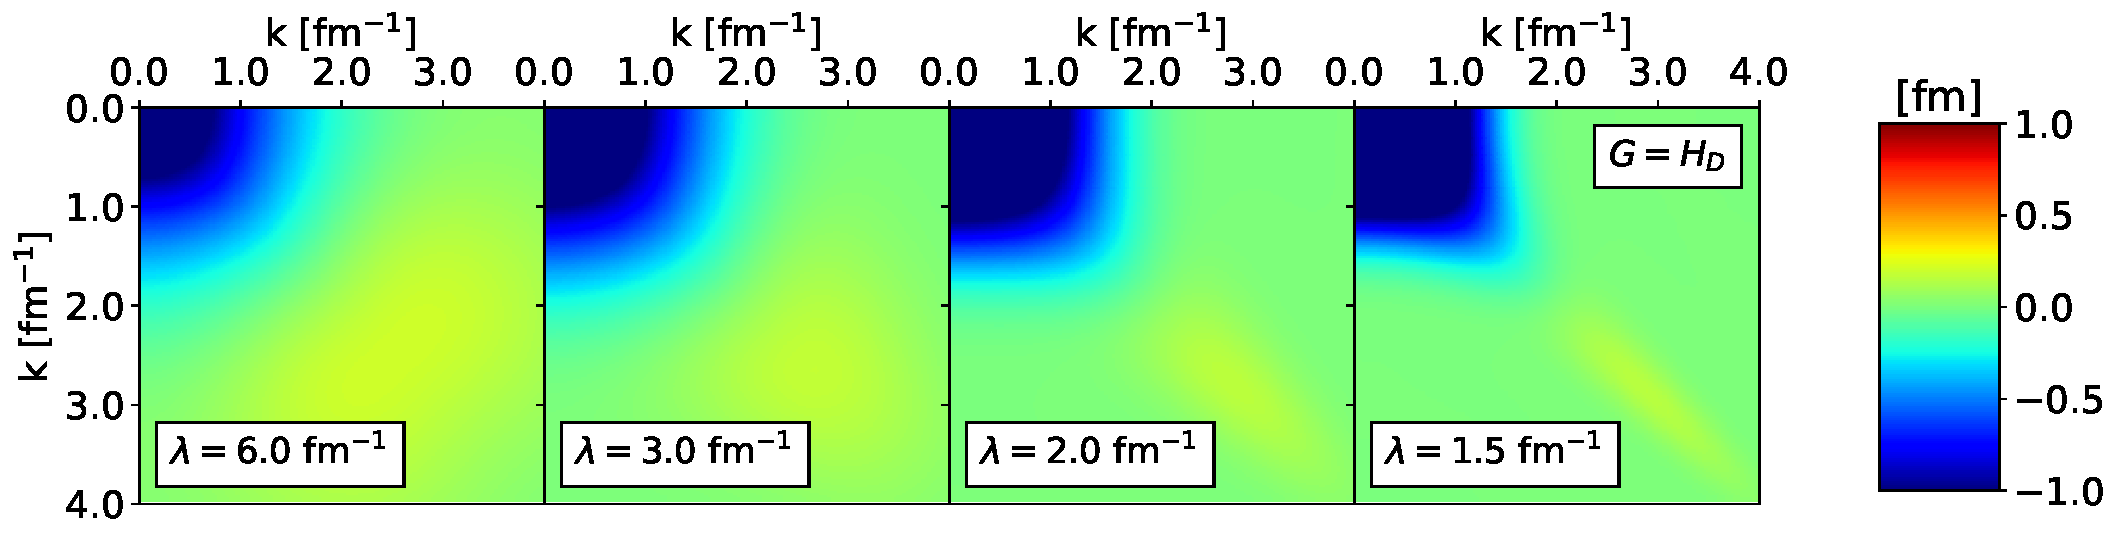
\includegraphics[clip,width=0.9\columnwidth]{SRG_potentials/potential_contours_kvnn106_3S1_Wegner_generator_label}%
	}
	
	\subfloat[]{%
	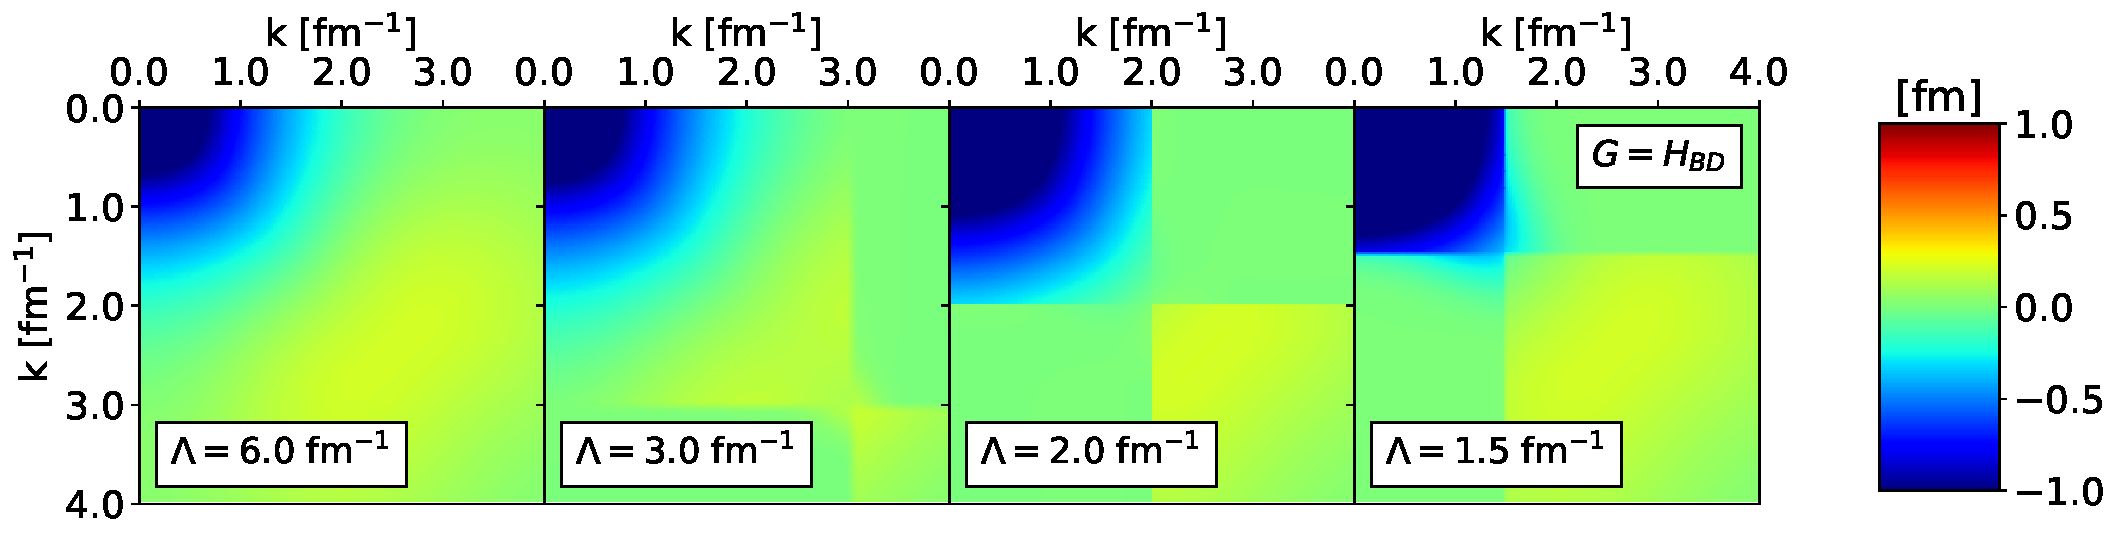
\includegraphics[clip,width=0.9\columnwidth]{SRG_potentials/potential_contours_kvnn106_3S1_Block-diag_generator_label}%
	}
	\caption{Matrix elements of the RKE N$^3$LO potential SRG-evolving right to left under transformations with Wegner (a) and block-diagonal (b) generators in the $^3$S$_1$ channel. Here, we use $\lambda$ for Wegner evolution in the top row and $\Lambda$ for block-diagonal evolution in the bottom row. For block-diagonal evolution, we fix $\lambda=1.5$ fm$^{-1}$.}
	\label{fig:potential_contours_3S1_RKE}
\end{figure}
%
\noindent{%
-- Fig.~\ref{fig:phase_shifts} shows the NN phase shifts of EM N$^3$LO, RKE N$^3$LO, and Gezerlis et al. N$^2$LO potentials in the $^1$S$_0$, $^3$S$_1$, and $^1$P$_1$ channels. In \cite{Dainton:2013axa}, it was found that phase equivalence up to some value of momentum $k$ implies matrix element equivalence up to the same value of $k$ in SRG-evolved potentials. We verify this conclusion by checking the matrix elements in Fig.~\ref{fig:potential_slices_1S0} where we see a collapse of the different potential matrix elements to the same line in the last column ($\lambda=1$ fm$^{-1}$). Note, Figs.~\ref{fig:potential_slices_1S0}-\ref{fig:potential_slices_1P1} show both Wegner and block-diagonal evolution where the solid lines correspond to the Wegner generator and dash-dotted to block-diagonal evolution. We see each generator collapses the potential to a different form because the low- and high-momentum matrix elements decouple in a different manner.
}
\\
-- In the $^3$S$_1$ channel, we see a slight deviation in the lowest momentum potential matrix element from EM N$^3$LO and the other two potentials. This is due to a minor difference in the deuteron binding energy ($\approx 1\%$ difference).
\\
-- The bottom row of Fig.~\ref{fig:potential_slices_1P1} shows $V(k,0.5)$ instead of $V(k,0)$ because the far off-diagonal matrix elements in the $^1$P$_1$ channel are all zero.
\begin{figure}[H]
	\centering
	\subfloat[]{%
	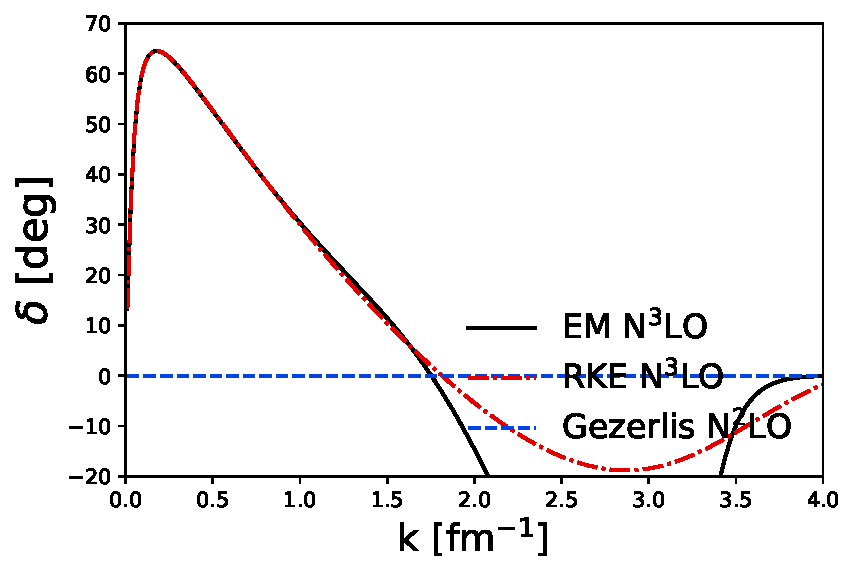
\includegraphics[clip,width=0.3\columnwidth]{SRG_observables/phase_shifts_1S0_kvnns_10_106_222}%
	}
	\quad
	\subfloat[]{%
	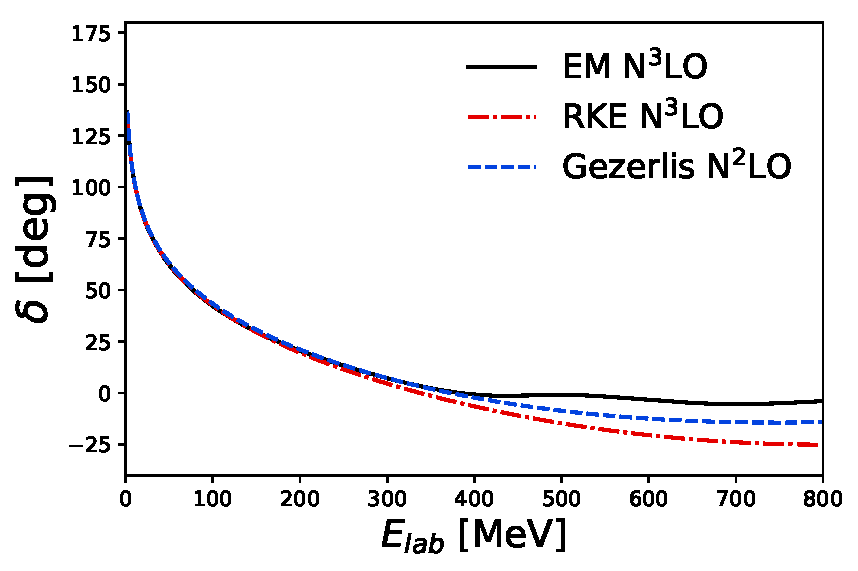
\includegraphics[clip,width=0.3\columnwidth]{SRG_observables/phase_shifts_3S1_kvnns_10_106_222}%
	}
	\quad
	\subfloat[]{%
	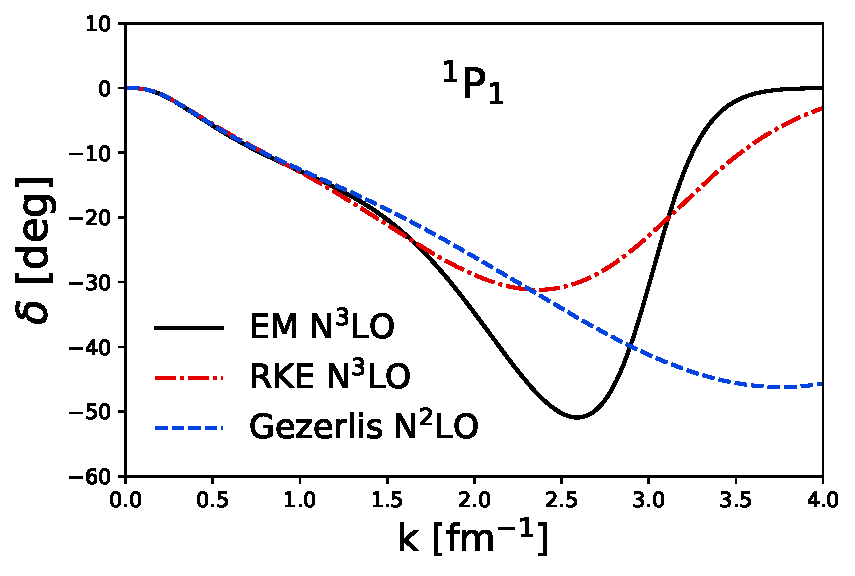
\includegraphics[clip,width=0.3\columnwidth]{SRG_observables/phase_shifts_1P1_kvnns_10_106_222}%
	}
	\caption{$^1$S$_0$ (a), $^3$S$_1$ (b), and $^1$P$_1$ (c) phase shifts for the EM N$^3$LO (solid black), RKE N$^3$LO (red dash-dotted), and Gezerlis et al. N$^2$LO (blue dashed) potentials.}
	\label{fig:phase_shifts}
\end{figure}
%
\begin{figure}[H]
	\centering
	\subfloat[]{%
	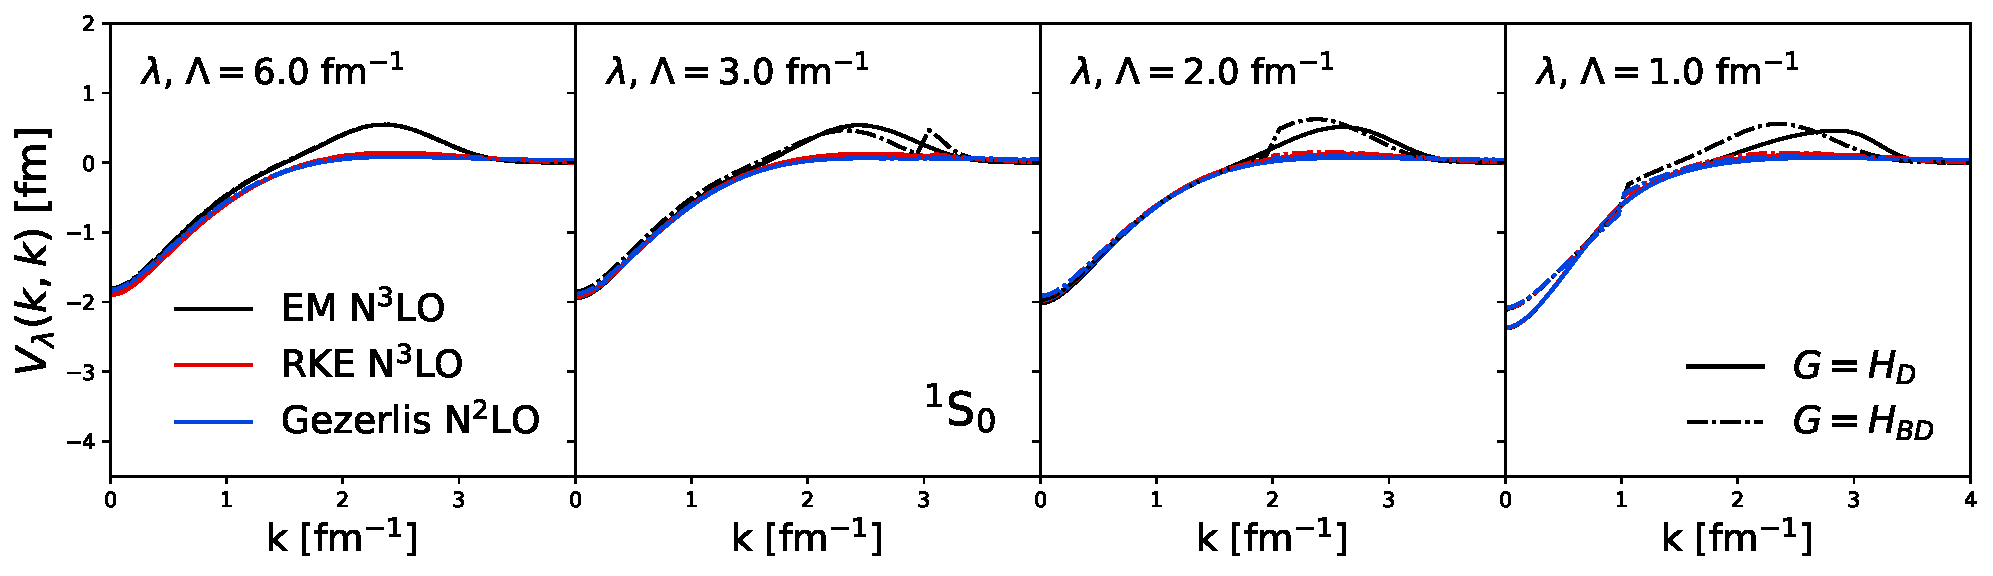
\includegraphics[clip,width=0.9\columnwidth]{SRG_potentials/potential_diag_1S0_kvnns_10_106_222_lamb1,0}%
	}
	
	\subfloat[]{%
	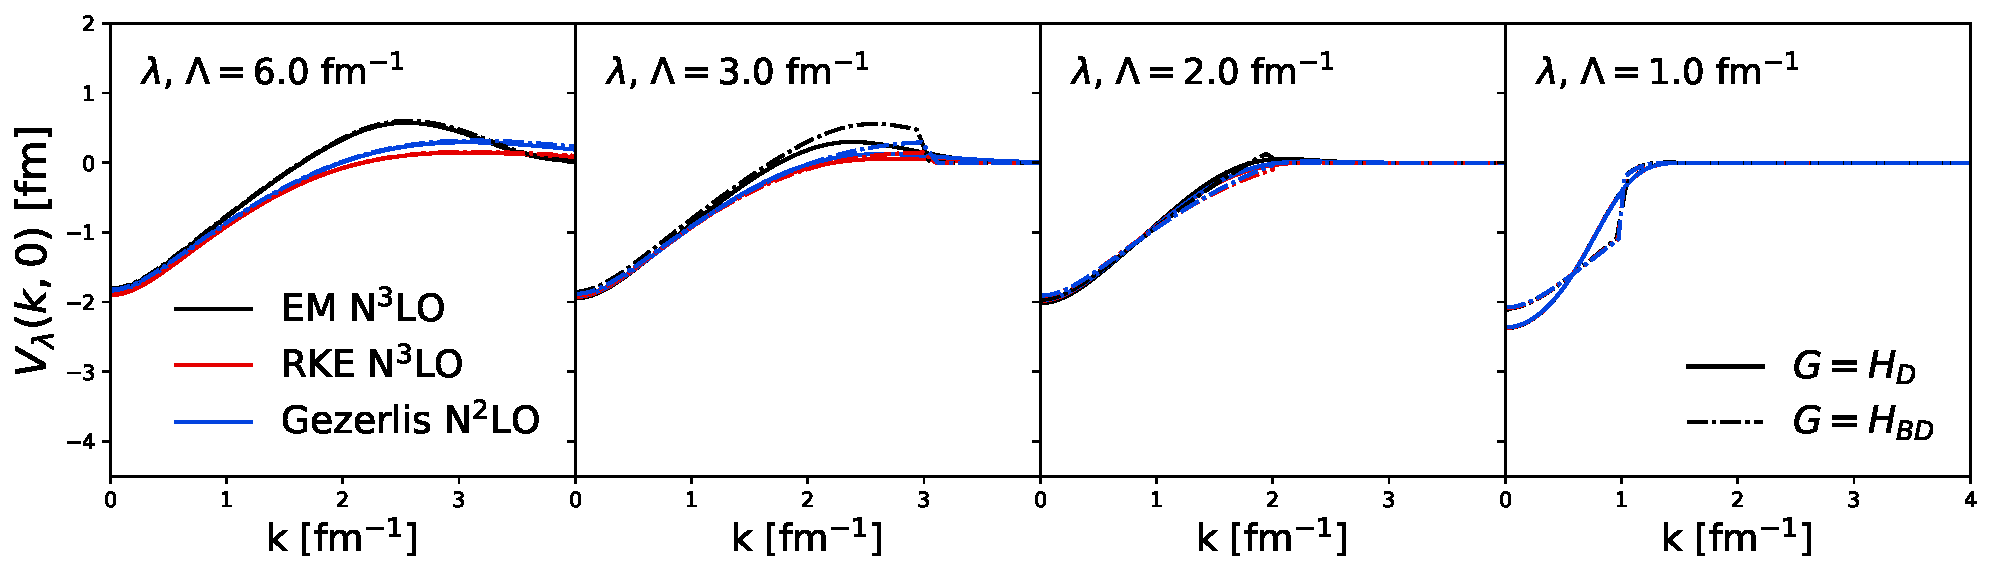
\includegraphics[clip,width=0.9\columnwidth]{SRG_potentials/potential_off-diag_1S0_kvnns_10_106_222_lamb1,0}%
	}
	\caption{Diagonal (a) and far off-diagonal (b) matrix elements of the EM N$^3$LO (black), RKE N$^3$LO (red) and Gezerlis et al. N$^2$LO (blue) potentials SRG-evolving right to left under transformations with Wegner (solid) and block-diagonal (dash-dotted) generators in the $^1$S$_0$ channel. Here, we use $\lambda$ for Wegner evolution and $\Lambda$ for block-diagonal evolution. For block-diagonal evolution, we fix $\lambda=1$ fm$^{-1}$.}
	\label{fig:potential_slices_1S0}
\end{figure}
%
\begin{figure}[H]
	\centering
	\subfloat[]{%
	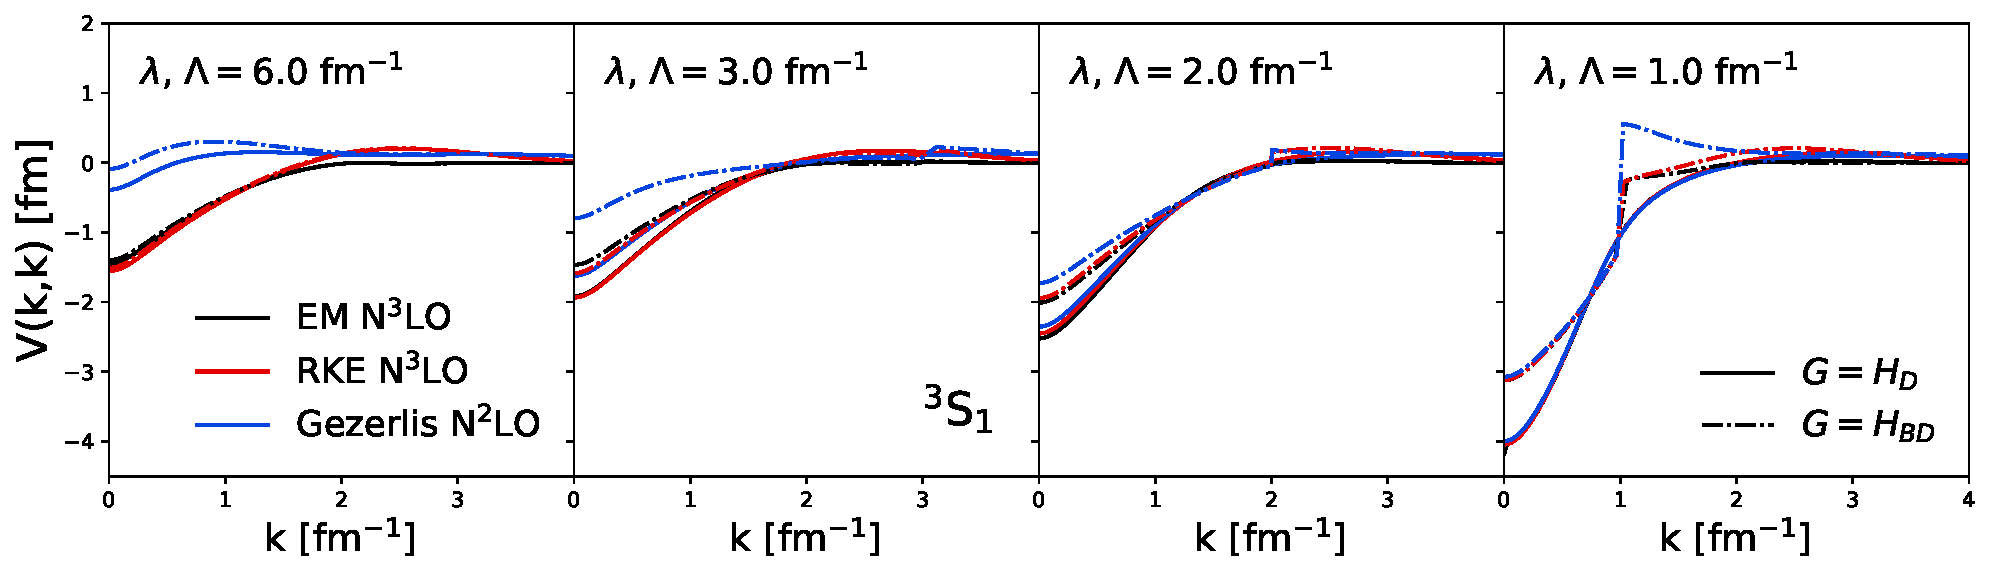
\includegraphics[clip,width=0.9\columnwidth]{SRG_potentials/potential_diag_3S1_kvnns_10_106_222_lamb1,0}%
	}
	
	\subfloat[]{%
	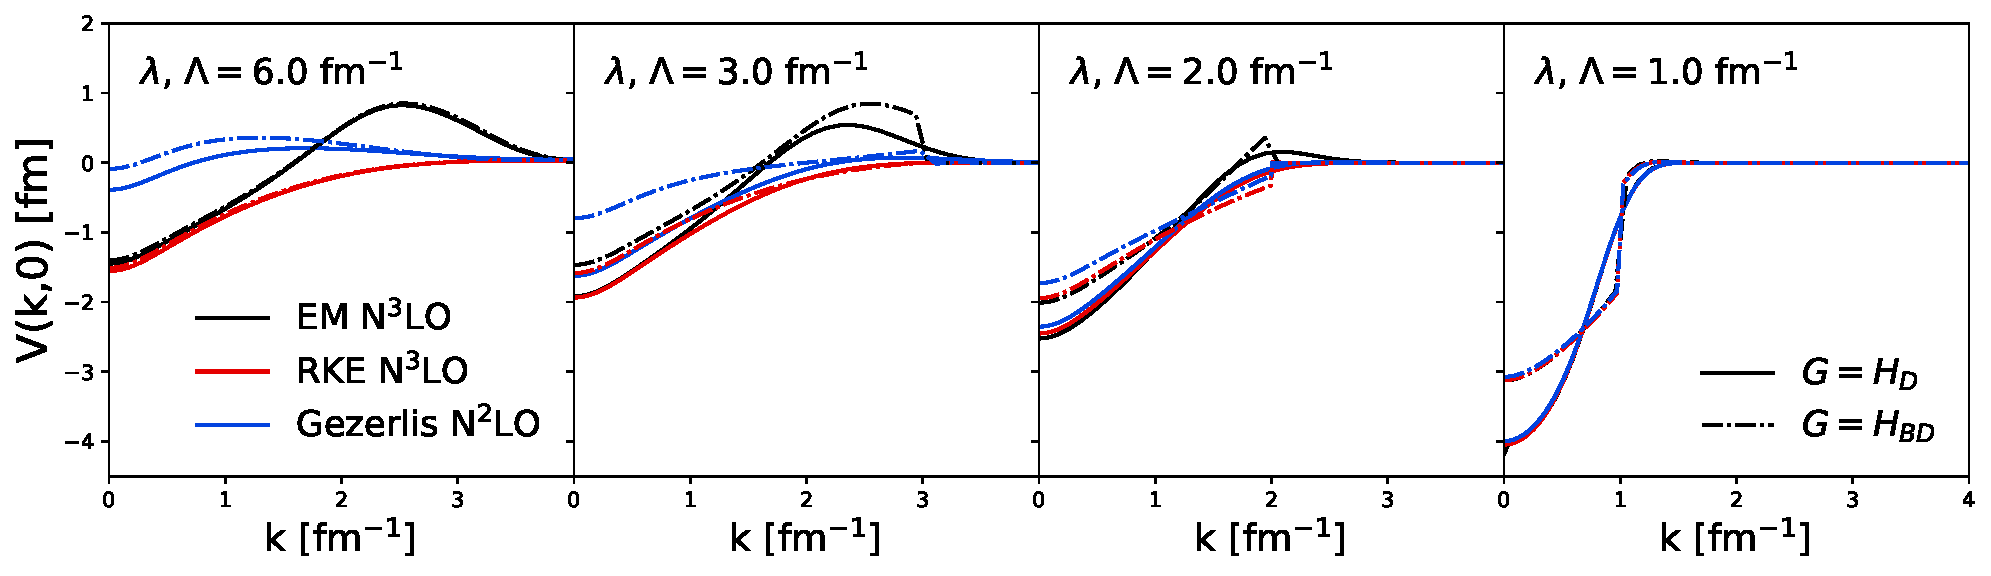
\includegraphics[clip,width=0.9\columnwidth]{SRG_potentials/potential_off-diag_3S1_kvnns_10_106_222_lamb1,0}%
	}
	\caption{Same as Fig.~\ref{fig:potential_slices_1S0} but in the $^3$S$_1$ channel.}
	\label{fig:potential_slices_3S1}
\end{figure}
%
\begin{figure}[H]
	\centering
	\subfloat[]{%
	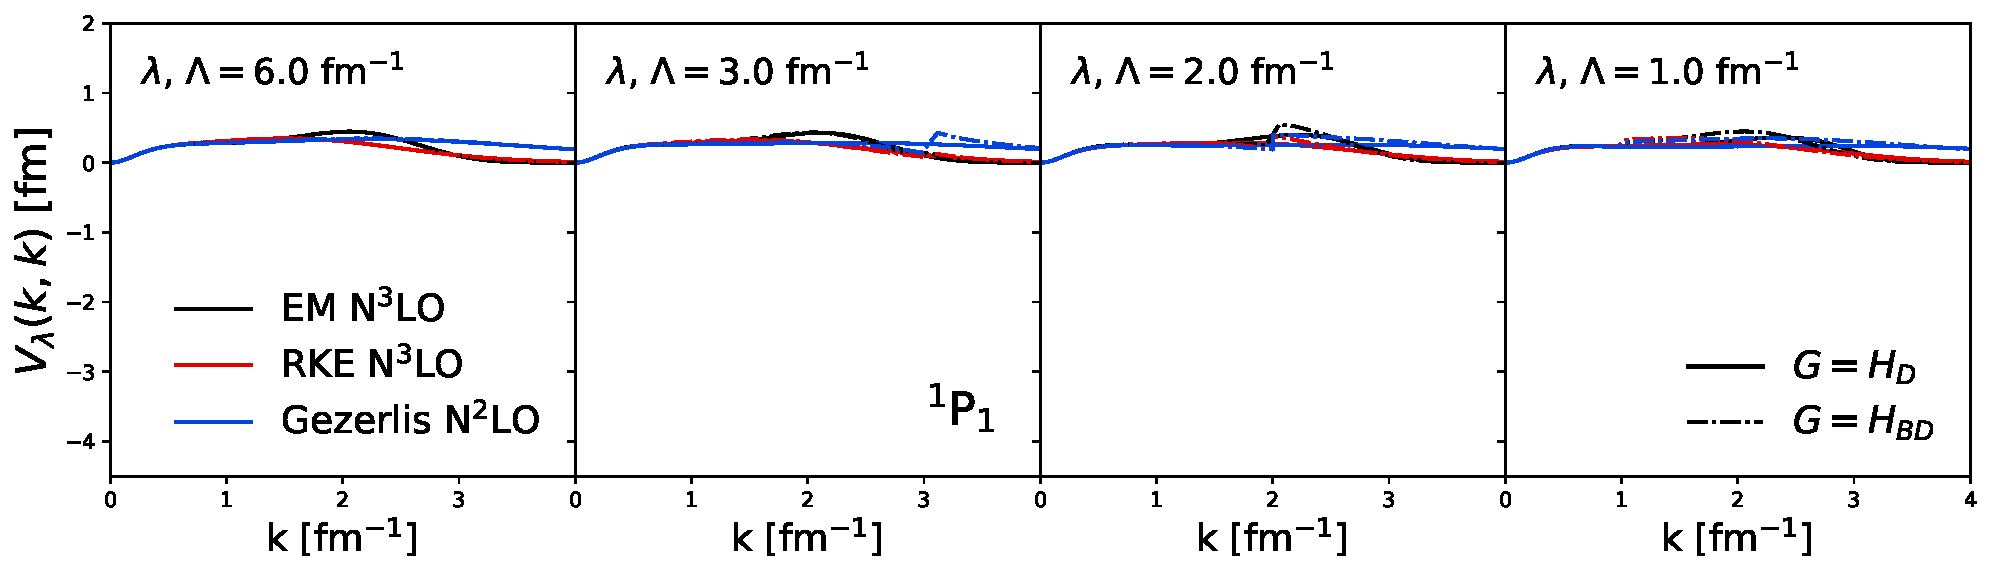
\includegraphics[clip,width=0.9\columnwidth]{SRG_potentials/potential_diag_1P1_kvnns_10_106_222_lamb1,0}%
	}
	
	\subfloat[]{%
	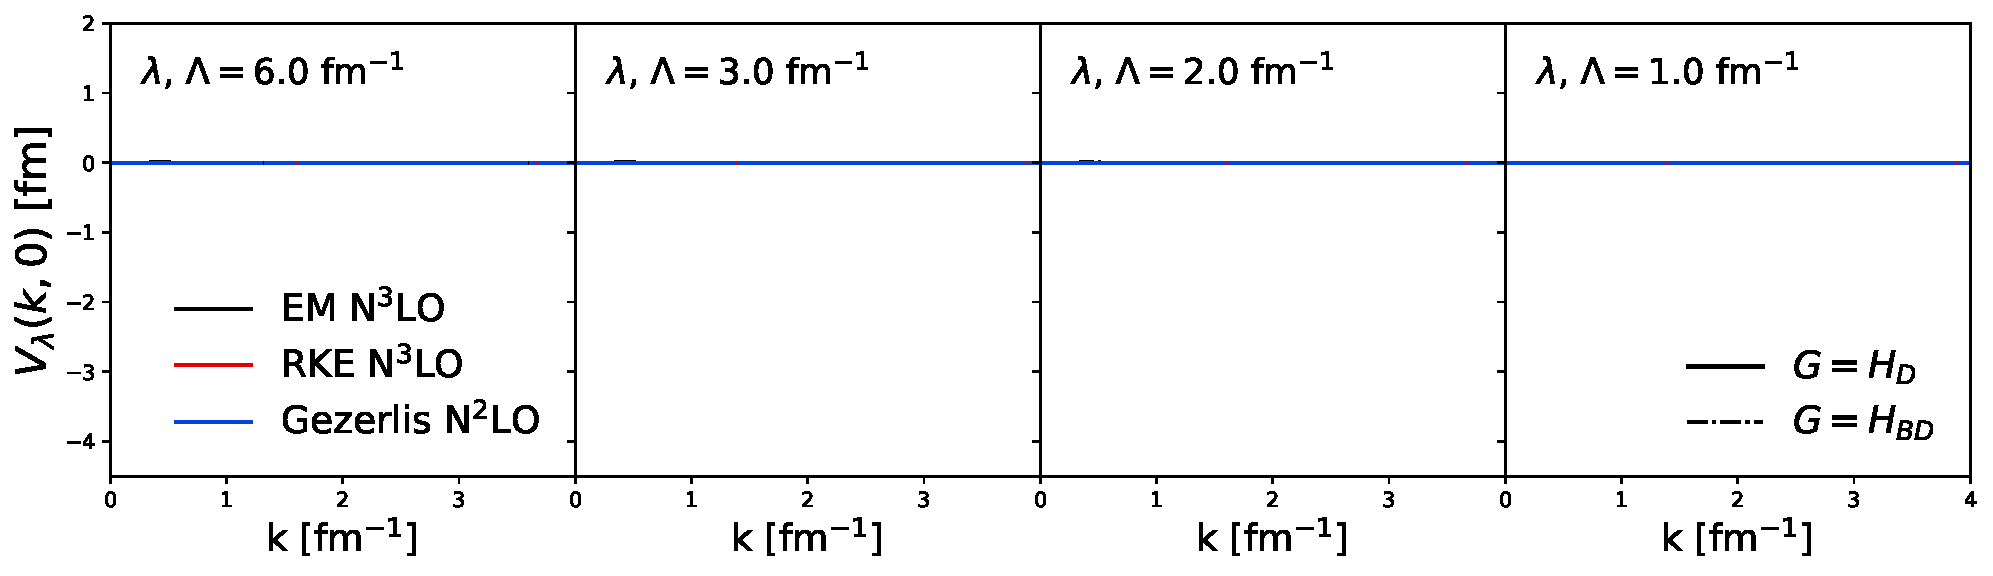
\includegraphics[clip,width=0.9\columnwidth]{SRG_potentials/potential_off-diag_1P1_kvnns_10_106_222_lamb1,0}%
	}
	\caption{Same as Figs.~\ref{fig:potential_slices_1S0} and \ref{fig:potential_slices_3S1} but in the $^1$P$_1$ channel.}
	\label{fig:potential_slices_1P1}
\end{figure}


%%%%%%%%%%%%%%%%%%%%%%%%%%%%%%%%%%%%%%%%%%%%%%%%%%%%%%%%%%%%%%%%%%%%%%%%%
\section{Evolution of other operators}
\label{sec:evolution_other_operators}


\noindent{%
-- SRG operator evolution for different potentials and generators.
}
\\
-- General questions to address: universality for operators, different generators.
\\
-- Give relevant equations. Unitary transformation equation.
\\
-- Momentum projection operator.
\\
-- Relevant equations: just the momentum projection operator in momentum-space.
%
\begin{itemize}
	\item Contours and general behavior: SRG transformation shifts strength of operator to low-momentum.
	\item Deuteron momentum distributions. Why does this make sense with the transformed operators?
	\item Diagonals and far off-diagonals. Universality.
	\item Same questions but with figures of the integrand.
\end{itemize}
%
\begin{figure}[H]
	\centering
	\subfloat[]{%
	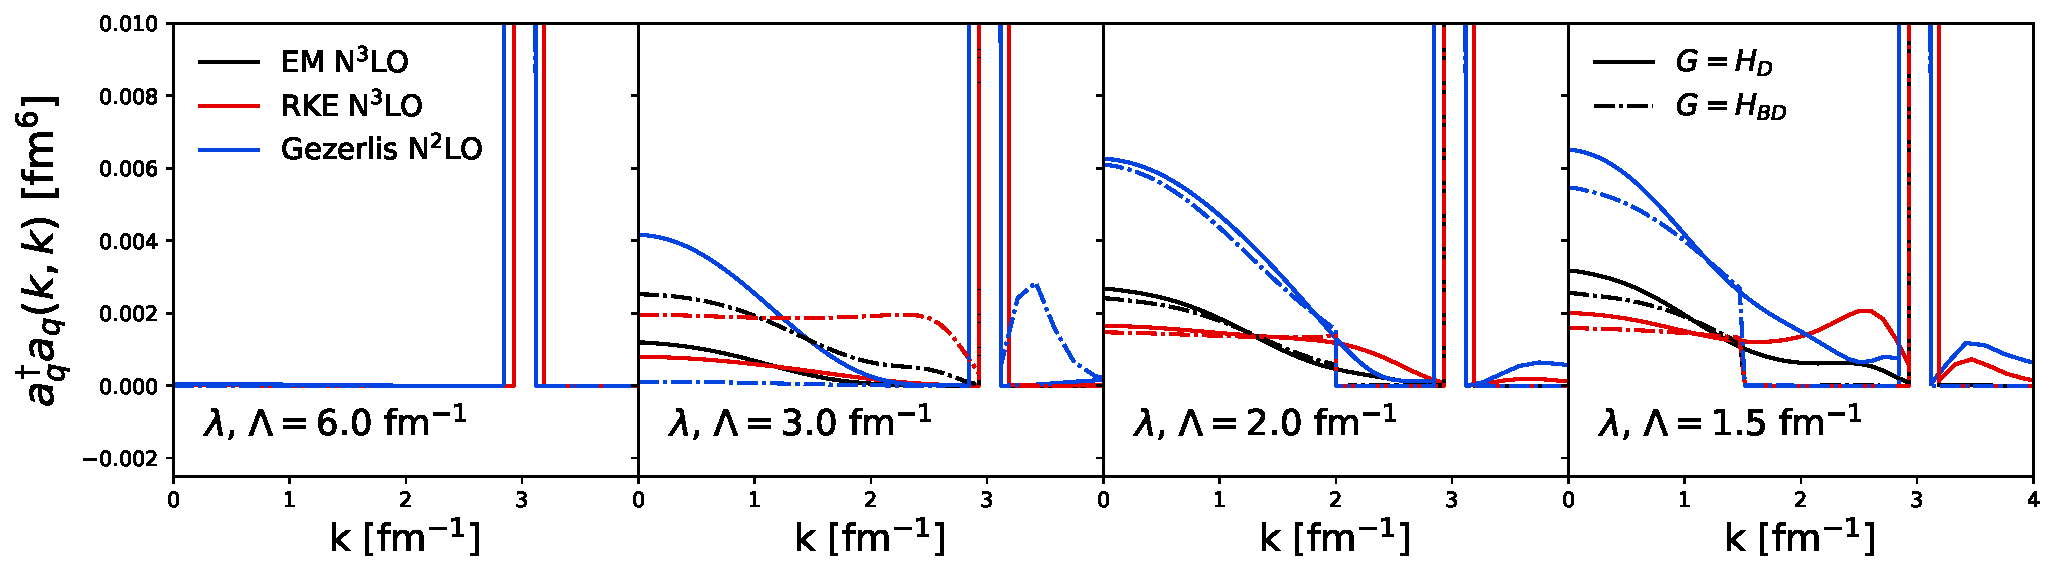
\includegraphics[clip,width=0.9\columnwidth]{SRG_operators/momentum_projection_diag_q3,00_3S1_kvnns_10_106_222_lamb1,5}%
	}
	
	\subfloat[]{%
	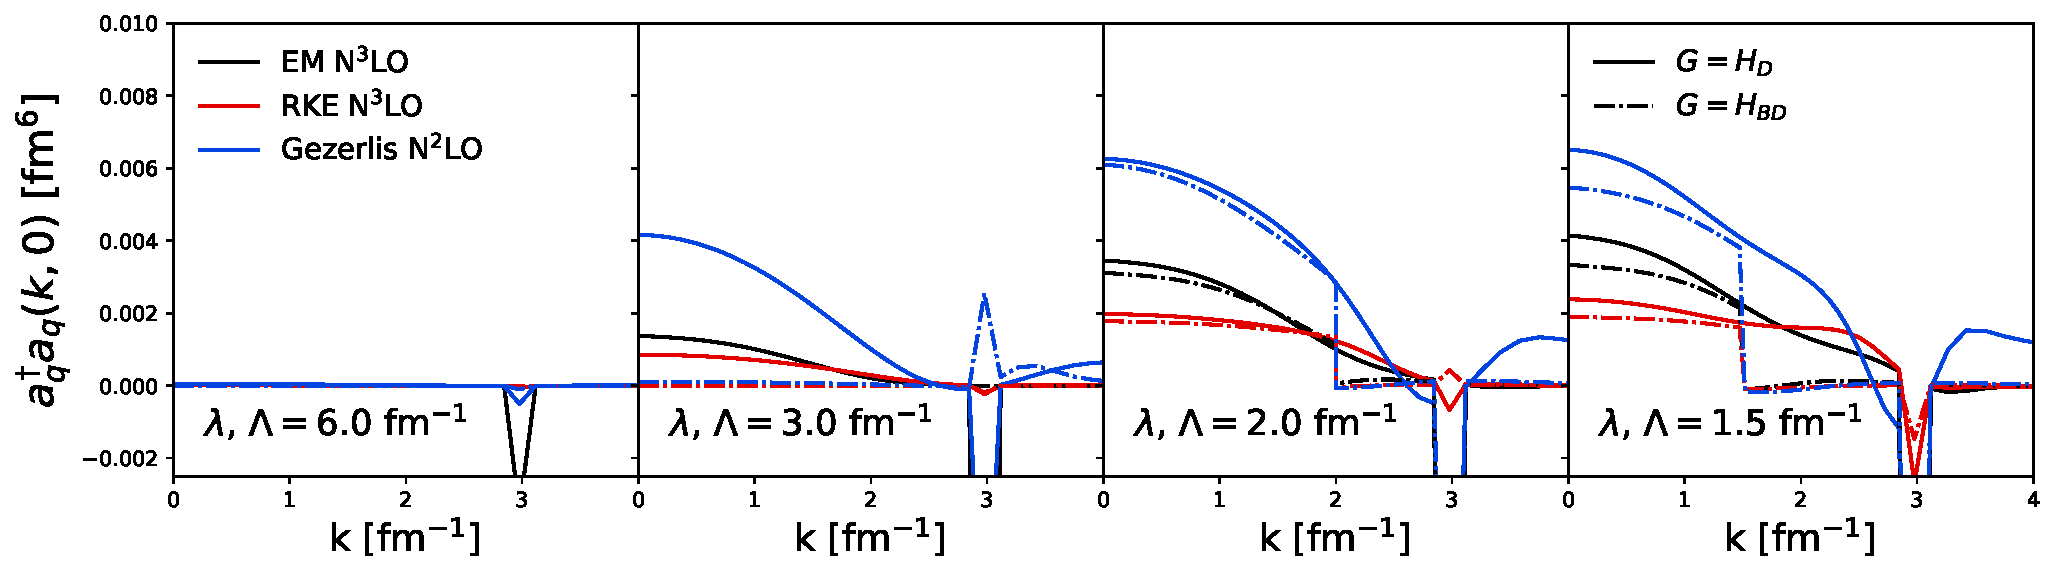
\includegraphics[clip,width=0.9\columnwidth]{SRG_operators/momentum_projection_off-diag_q3,00_3S1_kvnns_10_106_222_lamb1,5}%
	}
	\caption{Diagonal (a) and far off-diagonal (b) matrix elements of the momentum projection operator under SRG transformations with EM N$^3$LO (black), RKE N$^3$LO (red) and Gezerlis et al. N$^2$LO (blue) potentials evolving right to left with Wegner (solid) and block-diagonal (dash-dotted) generators in the $^3$S$_1$ channel. Here, we use $\lambda$ for Wegner evolution and $\Lambda$ for block-diagonal evolution. For block-diagonal evolution, we fix $\lambda=1.5$ fm$^{-1}$.}
	\label{fig:momentum_proj_3S1}
\end{figure}
%
-- Note, the unitary transformations and evolved wave functions for different potentials are not the same (at low momentum too) which implies that evolved operators cannot have the same universality property as the evolved potentials since they are dependent on the evolved wave functions.
\\
-- $\hat{r}^2$ operator.
\\
-- Relevant equations: operator in coordinate-space and Hankel transformation.


%%%%%%%%%%%%%%%%%%%%%%%%%%%%%%%%%%%%%%%%%%%%%%%%%%%%%%%%%%%%%%%%%%%%%%%%%
\section{High cutoffs and the Magnus expansion}
\label{sec:magnus_expansion}


\noindent{%
\textbf{High cutoffs}
}
\begin{itemize}
	\item Cutoff dependence in non-local LO (Wendt) potential.
	\item Band- and block-diagonal evolution and universality. Add figure analogous to Fig.~\ref{fig:potential_slices_3S1} but for $\Lambda=4$, $9$, and $20$ fm$^{-1}$.
	\item Spurious bound state(s).
	\item Transition to Magnus expansion.
\end{itemize}
%
\begin{figure}[H]
	\centering
	\subfloat[]{%
	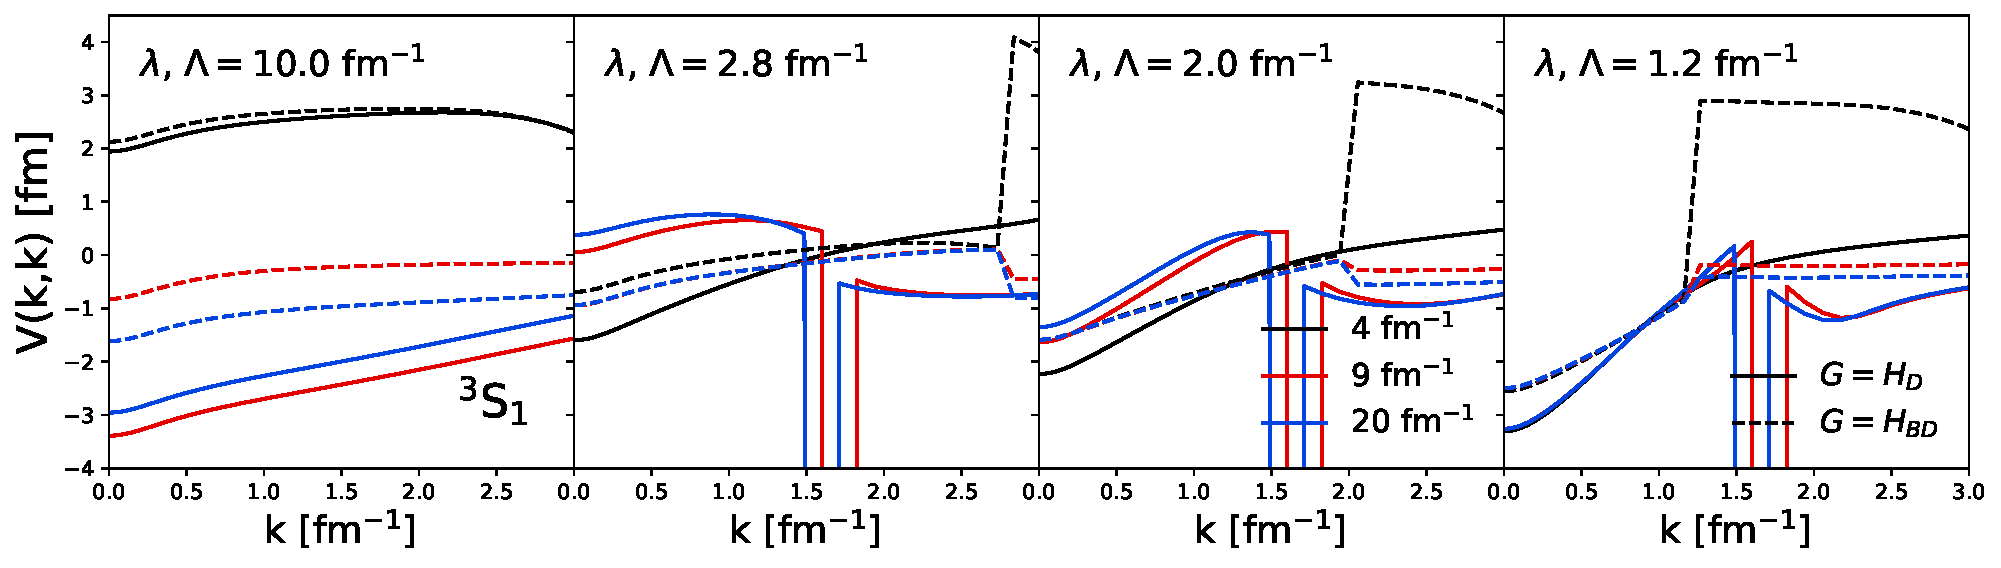
\includegraphics[clip,width=0.9\columnwidth]{SRG_potentials/potential_diag_3S1_kvnns_900_901_902_lamb1,2}%
	}
	
	\subfloat[]{%
	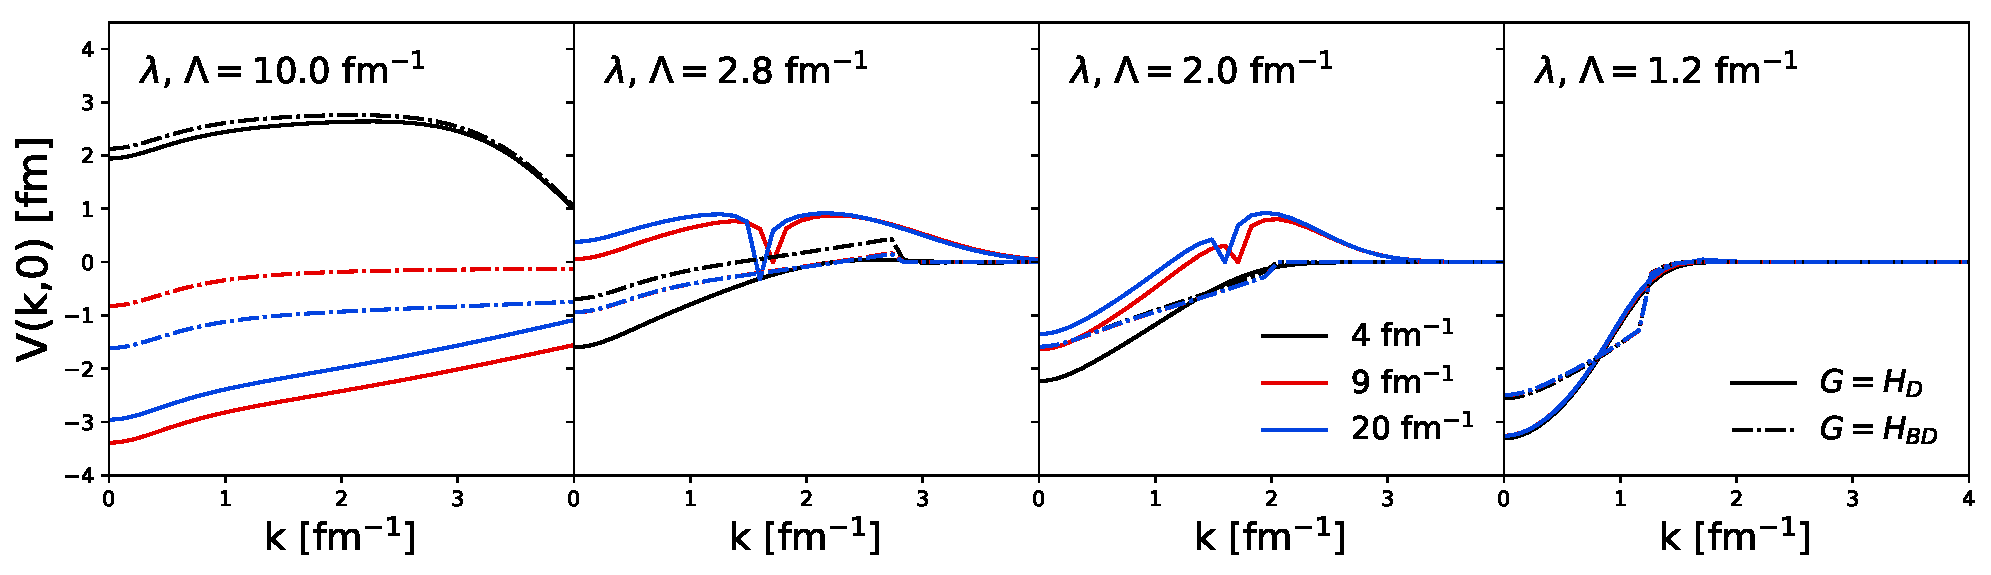
\includegraphics[clip,width=0.9\columnwidth]{SRG_potentials/potential_off-diag_3S1_kvnns_900_901_902_lamb1,2}%
	}
	\caption{Diagonal (a) and far off-diagonal (b) matrix elements of the non-local LO potentials at cutoffs $\Lambda=4$ (black), $9$ (red) and $20$ (blue) fm$^{-1}$ SRG-evolving right to left under transformations with Wegner (solid) and block-diagonal (dash-dotted) generators in the $^3$S$_1$ channel. Here, we use $\lambda$ for Wegner evolution and $\Lambda$ for block-diagonal evolution. For block-diagonal evolution, we fix $\lambda=1.2$ fm$^{-1}$.}
	\label{fig:potential_slices_high_cutoffs}
\end{figure}
%


% - - - - - - - - - - - - - - - - - - - - - - - - - - - - - - - - - - - - - - - - - - - - - - - - - - - - - - - - - - - - - - - - - - - - - - - - - - - - - - - - - - - - - - - - - - - - - - - - - - - - - - - - 
\subsection{Formalism}
\label{sec:magnus_expansion_formalism}


\noindent{%
-- Motivation: simplifies computational problem for evolving multiple operators, exact unitarity.
}
\\
-- We now consider the Magnus implementation.
\\
-- Mathematically speaking, the Magnus expansion is a method for solving an initial value problem associated with a linear ordinary differential equation (ODE).
\\
-- Formal details of the Magnus expansion are discussed in \cite{Blanes:2009ab}.
\\
-- We will introduce the Magnus expansion in the context of SRG evolving any operator.
\\
-- In an intermediate step in deriving Eqn. (\ref{eq:srg_flow}), we have a linear ODE for $U(s)$,
%
\begin{eqnarray}
	\label{eq:unitary_trans}
	\frac{dU(s)}{ds} = \eta(s) U(s).
\end{eqnarray}
%
-- Magnus showed that one can solve the following equation with a solution $U(s)=e^{\Omega(s)}$ where $\Omega(s)$ is expanded as a power series, $\sum_{n}^{\infty} \Omega_n$ (referred to as the Magnus expansion or Magnus series).
\\
-- The terms of the series are given by integral expressions involving $\eta(s)$ (again, see \cite{Blanes:2009ab, Magnus:1954zz} for details).
\\
-- For our case, we focus on the formally exact derivative of $\Omega(s)$,
%
\begin{eqnarray}
	\label{eq:magnus_omega}
	\frac{d\Omega(s)}{ds} = \sum_{k=0}^{\infty} \frac{B_k}{k!} ad_{\Omega}^{k}(\eta),
\end{eqnarray}
%
where $B_k$ are the Bernoulli numbers, $ad_{\Omega}^{0}(\eta)=\eta(s)$, and $ad_{\Omega}^{k}(\eta)=[\Omega(s),ad_{\Omega}^{k-1}(\eta)]$.
\\
-- We integrate this differential equation to find $\Omega(s)$ and evaluate the unitary transformation directly.
\\
-- Then the evolved operator can be evaluated with the BCH formula:
%
\begin{eqnarray}
	\label{eq:bch}
	O(s) = e^{\Omega(s)} O e^{-\Omega(s)} = \sum_{k=0}^{\infty} \frac{1}{k!} ad_{\Omega}^{k}(O).
\end{eqnarray}
%
-- As $k \rightarrow \infty$ in both sums in Eqns. (\ref{eq:magnus_omega}) and (\ref{eq:bch}) the Magnus transformation matches the SRG transformation exactly.
\\
-- We investigate several truncations $k_{max}$ in Eqn. (\ref{eq:magnus_omega}) and take many terms, $k_{max} \sim 25$, in Eqn. (\ref{eq:bch}).
\\
\textcolor{red}{%
-- Here or earlier (for the following bullets)? Better to motivate the Magnus in the introduction or easier to explain given mathematical detail?
}
\\
-- There are significant advantages in the Magnus implementation.
\\
-- In the typical approach, the numerical error associated with solving the flow equation affects the accuracy of the observables for the evolved operator.
\\
-- Therefore, one must use a high-order ODE solver in integrating the flow equation (\ref{eq:srg_flow}).
\\
-- In the Magnus implementation, unitarity is guaranteed by the form of $U(s)$; in fact, one could solve Eqn. (\ref{eq:magnus_omega}) with a simple first-order Euler step-method keeping the same observables while decoupling the operator as desired.
\\
-- This offers a decent computational speed-up by avoiding a high-order solver.
\\
-- In this paper, we demonstrate this advantage by applying the Magnus implementation using the first-order Euler step-method.
\\
-- The second major advantage involves the evolution of multiple operators.
\\
-- In many other situations, one may be interested in evolving several operators at a time.
\\
-- In the SRG procedure, we would have another set of coupled equations in Eqn. (\ref{eq:srg_flow}), drastically increasing memory usage.
\\
-- Each additional operator increases the set of equations - say $N$ equations - by another factor of $N$.
\\
-- In the Magnus, one only needs $\Omega(s)$ to consistently evolve several operators.
\\
-- We avoid the cost in memory by directly constructing $U(s)=e^{\Omega(s)}$.
\\
-- This is especially useful in IMSRG calculations where the model space can be very large.
\\
-- In the next section, we discuss results from Magnus-evolved large-cutoff potentials focusing on the flow of the potential, observables, and operator evolution.


% - - - - - - - - - - - - - - - - - - - - - - - - - - - - - - - - - - - - - - - - - - - - - - - - - - - - - - - - - - - - - - - - - - - - - - - - - - - - - - - - - - - - - - - - - - - - - - - - - - - - - - - - 
\subsection{Results}
\label{sec:magnus_expansion_results}


\noindent{%
-- Comparison to Wendt problem.
}
\\
-- Implications for IMSRG.
\\
-- Discussion on how the block-diagonal generator handles spurious bound states. Where they are ``decoupled'' in the matrix compared to Wegner. One figure to show this?
%
\begin{figure}[H]
	\centering
	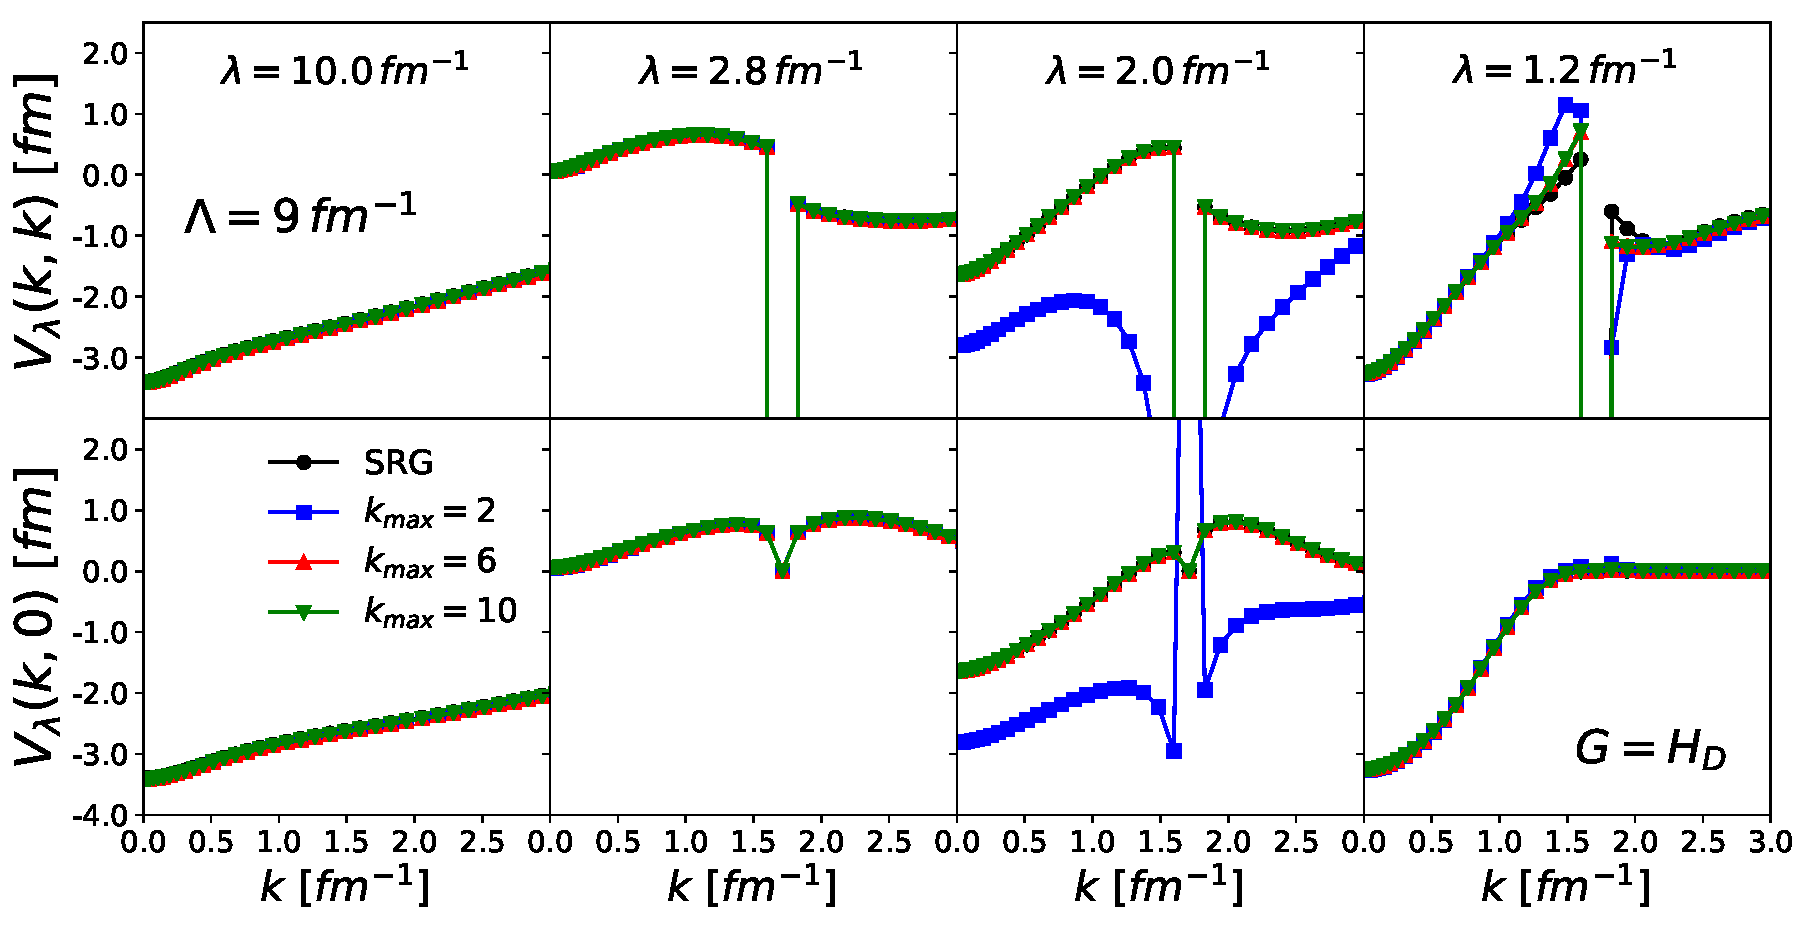
\includegraphics[clip,width=0.9\columnwidth]{Magnus/potential_diagonals_offdiags_kvnn901_Wegner}%
	%\caption{Caption.}
	\label{fig:potential_slices_high_cutoffs_Wegner}
\end{figure}
%
\begin{figure}[H]
	\centering
	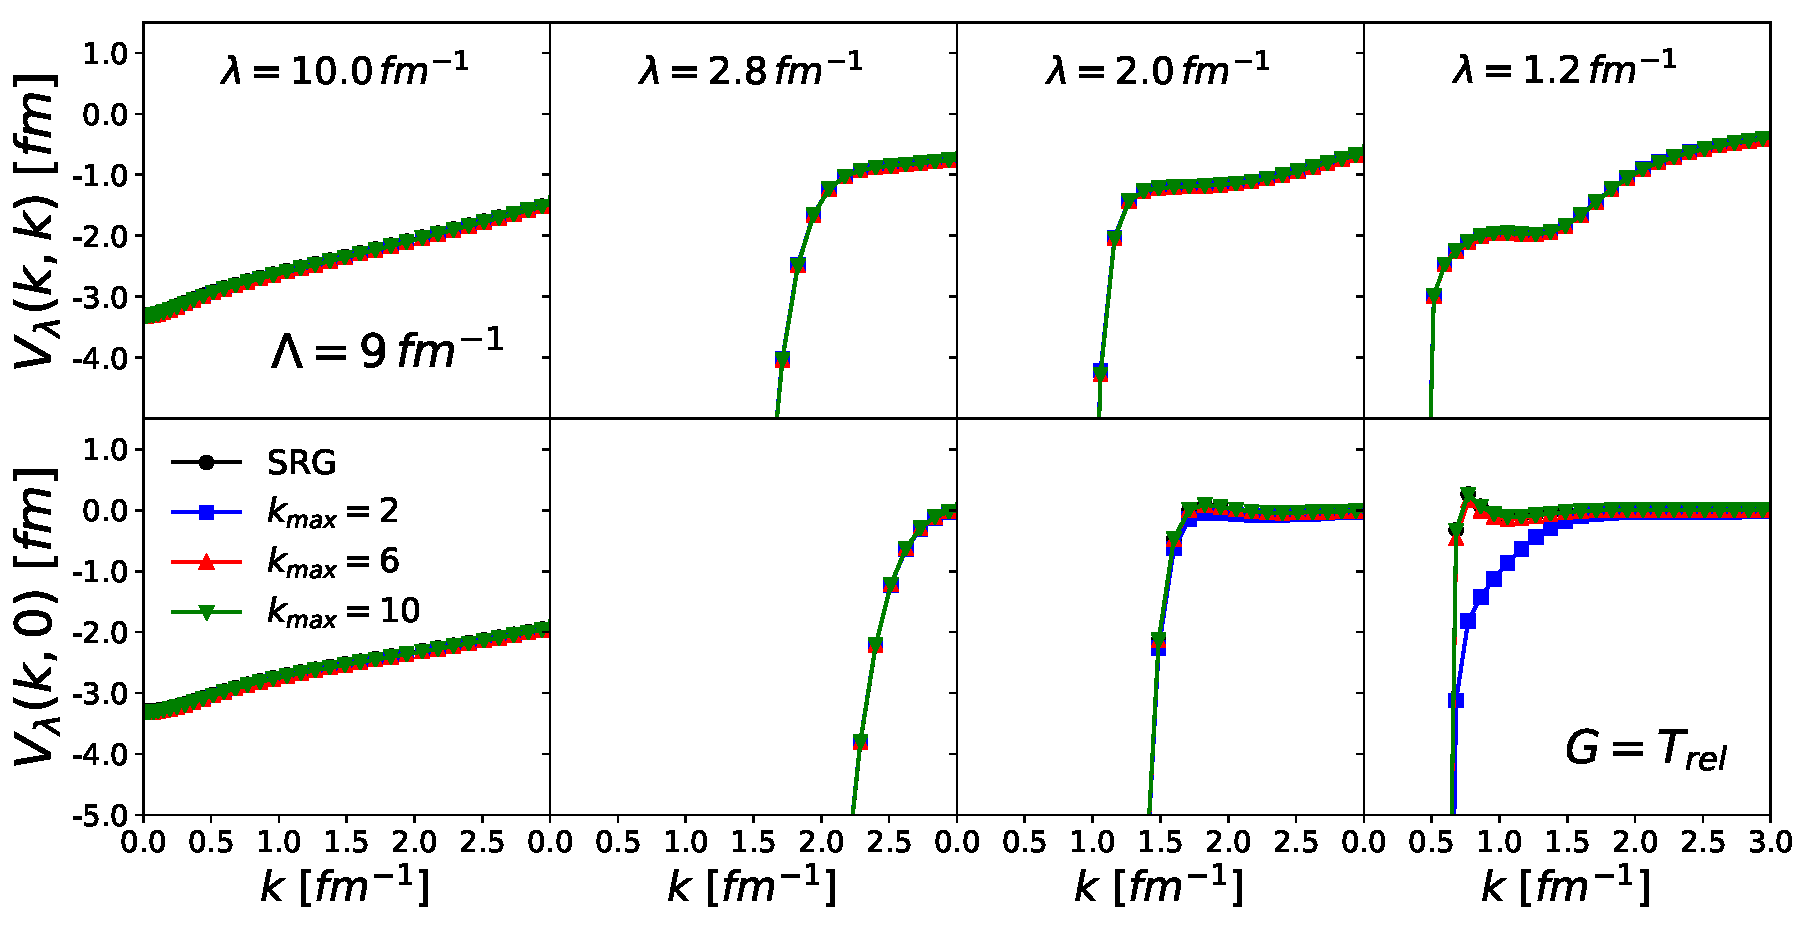
\includegraphics[clip,width=0.9\columnwidth]{Magnus/potential_diagonals_offdiags_kvnn901_T}%
	%\caption{Caption.}
	\label{fig:potential_slices_high_cutoffs_T}
\end{figure}
%


%%%%%%%%%%%%%%%%%%%%%%%%%%%%%%%%%%%%%%%%%%%%%%%%%%%%%%%%%%%%%%%%%%%%%%%%%
\section{Conclusion}
\label{sec:conclusion}


\noindent{%
-- Summary.
}
\\
-- Outlook.


%%%%%%%%%%%%%%%%%%%%%%%%%%%%%%%%%%%%%%%%%%%%%%%%%%%%%%%%%%%%%%%%%%%%%%%%%


\bibliography{../tropiano_bib}

\end{document}